\chapter{Hydrogenated Graphene}
When a Hydrogen adatom is deposited on graphene its $s$ orbital and the $p_z$ orbital from the Carbon below hybridize forming a \ac{bab} pair of states. The effective hopping\footnote{combination of $V_{sp\sigma}\sim\SI{-7}{\eV}$ (main contribution) and $V_{ss\sigma}\sim\SI{8}{\eV}$.} between the $H$ and the $C$ is around $t\simeq\SI{12}{\eV}$, so in the simplest possible model of a \ac{bab} pair we could expect that the resulting levels are far away from the low energy region as shown in figure \ref{bab}. If we look at the band structure of graphene (figure \ref{Gbands}) we can see that close to the \ac{bab} energies some sigma states appear.
%~~~~~~~~~~~~~~~~~~~~~~~~~~ FIGURE ~~~~~~~~~~~~~~~~~~~~~~~~~%
\begin{figure}[h!]
\centering
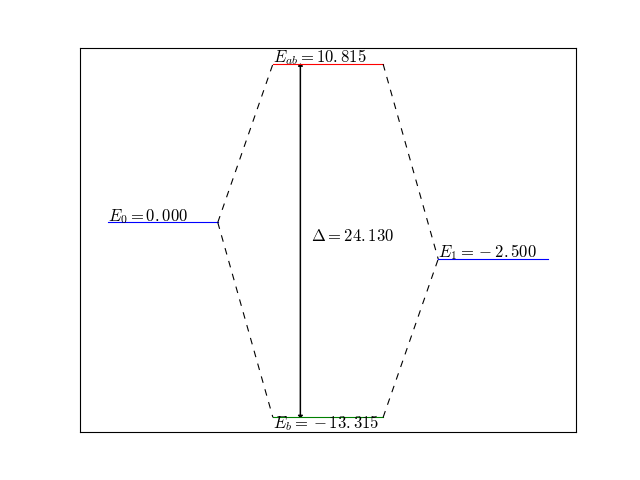
\includegraphics{chapter05/figures/bonding_antibonding.png}
% \vspace{-5pt}
\caption{Bonding-antibonding pair of states for a $s$ and a $p_z$ orbital with a hopping of $t\sim\SI{12}{\eV}$. Notice that the resulting states lie far above (and bellow) from the Fermi energy, $E_f=0$.}
\label{bab}
\end{figure}
\FloatBarrier
%~~~~~~~~~~~~~~~~~~~~~~~~~~~~~~~~~~~~~~~~~~~~~~~~~~~~~~~~~~~%
Of course there are there are other processes that would complicate this naive (and rather simplistic) picture, but in essence we can expect that the hybridization of the $s$ orbital and the $p_z$ should results in the effective removal of one $p_z$ orbitals in the low energy regime.\\

As explained in chapter \ref{ch:graphene} \blue{if we restrict ourselves to the low energy limit} graphene is a bipartite lattice, and since it is naturally at half filling. According to the Lieb's theorem if there is an imbalance in one of the sublattices \red{Extend. Lieb theorem. E=0 states...}\\

This one-orbital model will not be enough to describe the effective hyperfine interaction since it lacks the $H$ $s$ orbital in its description, for this reason we will keep a complementary description using a more complete basis for the system.

When using the whole $n=2$ set of orbitals, namely $s$, $p_x$, $p_y$, $p_z$, the general description does not change heavily, the zero energy state is no longer required to be exactly at $E=0$, but an in-gap state appears by introducing a H adatom.
%~~~~~~~~~~~~~~~~~~~~~~~~~~ FIGURE ~~~~~~~~~~~~~~~~~~~~~~~~~%
\begin{figure}[h!]
\centering
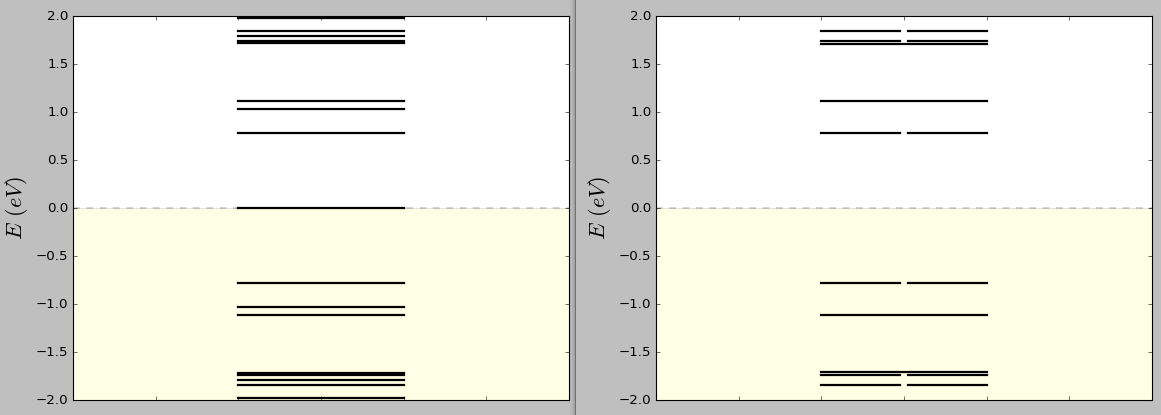
\includegraphics{chapter05/figures/spectrum1orb.png}
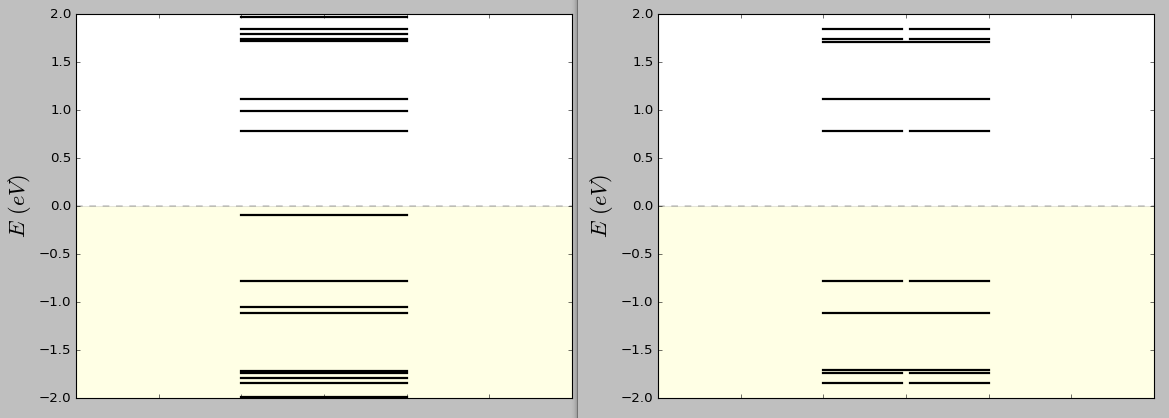
\includegraphics{chapter05/figures/spectrum4orb.png}
\vspace{-5pt}
\caption{Comparison of the 1 orbital model and the 4 orbital model. Spectrum of a 42 $C$ atoms island with (left) and without (right) H adatom.}
\label{Label}
\end{figure}
\FloatBarrier
%~~~~~~~~~~~~~~~~~~~~~~~~~~~~~~~~~~~~~~~~~~~~~~~~~~~~~~~~~~~%
The thing


\section{Finite systems}
We are going to begin studying the properties of a Hydrogen adatoms on graphene islands, taking special interest in the study of the hyperfine coupling of the $H$.

It is well known that depending in the edge of the islands (armchair, zigzag), the graphene islands may present a zero energy state in its spectrum according to the Lieb's theorem. Namely the zig-zag (triangular or hexagonal) islands do present zero energy states while armchair islands do not present such states.
We will focus on armchair islands, decorated with a Hydrogen adatom.


\subsection{Electronic states}
To get a general idea of the system we will use a \ac{tb} Hamiltonian considering only $p_z$ orbitals. As we stated before the introduction of a $H$ adatom results in the effective removal of one of the sites at low energy (where this 1-orbital description holds). According to Lieb's Theorem, since graphene is a bipartite lattice at half filling, a zero energy state is expected to appear.

We will use hexagonal armchair islands since their spectrum is always gapped and then remove one of the central atoms.

%~~~~~~~~~~~~~~~~~~~~~~~~~~ FIGURE ~~~~~~~~~~~~~~~~~~~~~~~~~%
\begin{figure}[h!]
\centering
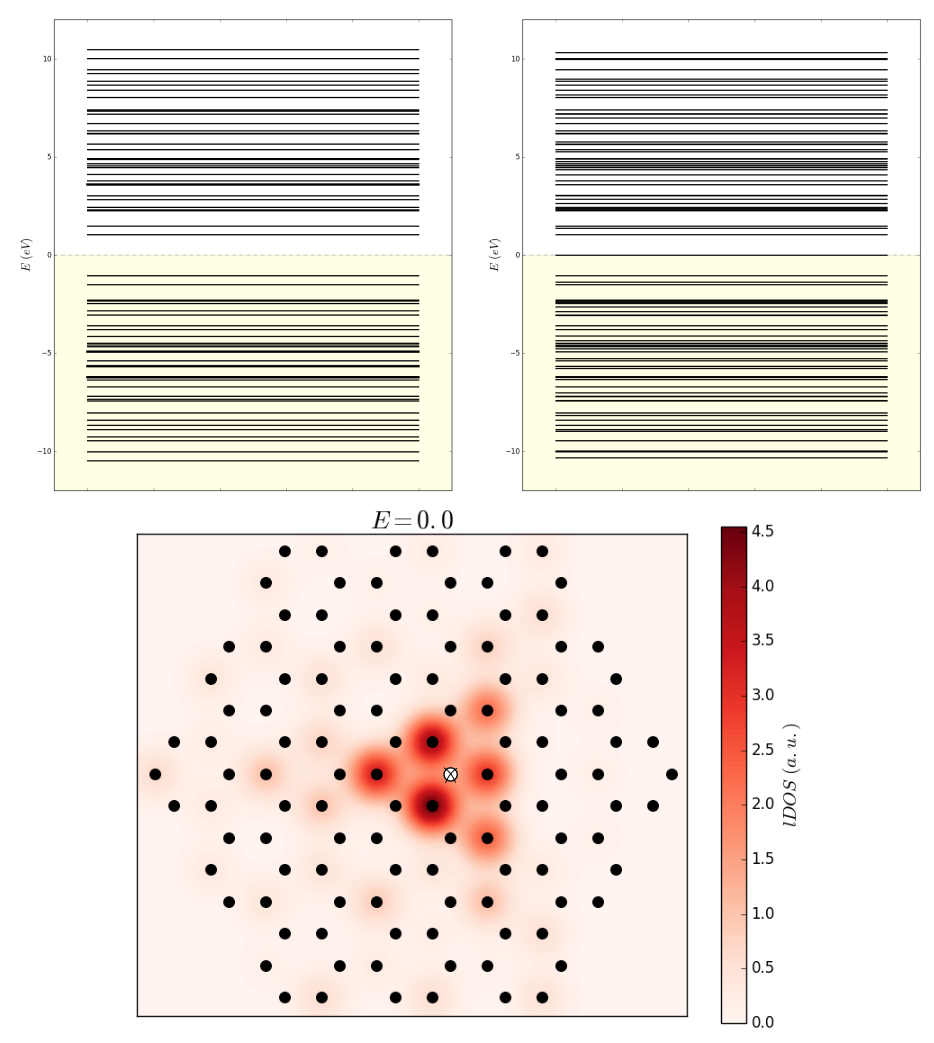
\includegraphics{chapter05/figures/espectro.png}
\vspace{-5pt}
\caption{$a)$ energy spectrum for a pristine island and an island with a vacancy, the width of the lines is proportional to the degeneracy of each state. $b)$ \ac{lDOS} of an armchair graphene island with a vacancy depicted by the white dot at $E=0$.}
\label{spectrum1}
\end{figure}
\FloatBarrier
%~~~~~~~~~~~~~~~~~~~~~~~~~~~~~~~~~~~~~~~~~~~~~~~~~~~~~~~~~~~%

As seen in figure \ref{spectrum1}, the introduction of a vacancy in graphene results in a zero energy state whose wave function is mostly localized in the 3-6 atoms closest to the vacancy. Also, as expected from Lieb's Theorem this state is sublattice polarized (its wave function vanishes in the sites belonging to the same sublattice as the vacancy).

This low energy model is enough to get an idea of the electronic behavior of the system, but in order to study the hyperfine interaction we need a more detailed description.

In particular the behavior of the $s$ orbital of the chemisorbed Hydrogen will play a crucial role in the magnitude of the hyperfine coupling.\\

We will consider now a \ac{sk} Hamiltonian as described in section \ref{sec:SK} with $s$, $p_x$, $p_y$ and $p_z$ orbitals for the $C$ atoms and $s$ orbital for the $H$ atoms.

If we repeat the previous process we would get tons of close-to-zero states corresponding to the dangling bonds of the $C$ atoms in the borders. To avoid this inconvenience we passivate the edge adding $H$ atoms so the $p_x$ and $p_y$ orbitals can keep their $sp^2$ hybridization. The result in this case is completely analogous, but with $\sim\times4$ more states.\\

%~~~~~~~~~~~~~~~~~~~~~~~~~~ FIGURE ~~~~~~~~~~~~~~~~~~~~~~~~~%
\begin{figure}[h!]
\centering
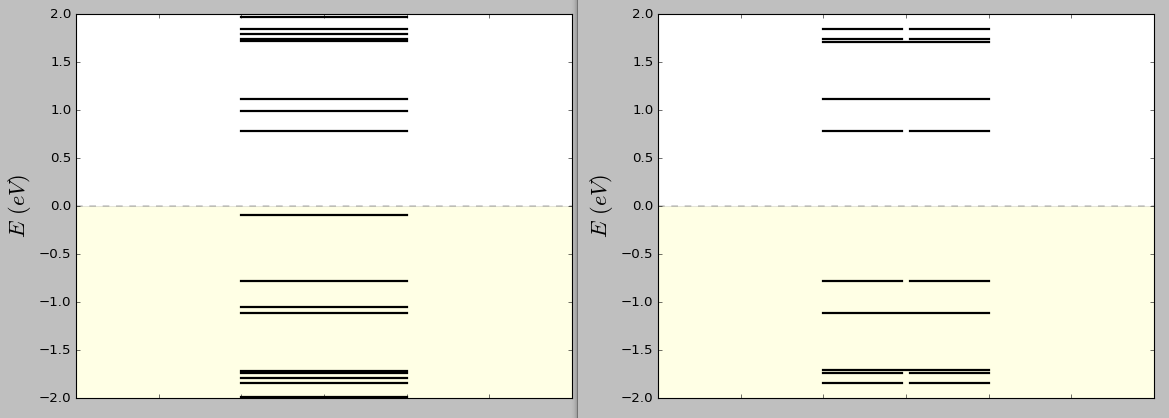
\includegraphics[width=0.9\textwidth]{chapter05/figures/spectrum4orb.png}
\vspace{-5pt}
\caption{Spectrum with and without $H$ adatom on an armchair island with 42 $C$ atoms.}
\label{spectrum4}
\end{figure}
\FloatBarrier
%~~~~~~~~~~~~~~~~~~~~~~~~~~~~~~~~~~~~~~~~~~~~~~~~~~~~~~~~~~~%

The main difference is that the zero-energy state is no longer at $E=0$. This shift is due to the finite on-site energy of the $H$ atom and the finite hopping between orbitals. Since now we are considering the full range of energies the Hydrogen is no longer a vacancy and the Lieb's theorem does not apply. Nevertheless we will refer to the in-gap state as the zero-energy state even when it is not strictly  at $E=0$.

The spatial localization of the zero-energy state is quite similar, although if we examine the wave function it is not strictly sublattice polarized, yet it is apparent that the 1 orbital model is enough to describe the general features.

As described in sec \ref{sec:hyperfine}, to calculate the effective hyperfine coupling we just have to project the zero energy state in the $1s$ Hydrogen orbital.
\begin{equation}
\mathcal{A} = |\braket{\phi_{1s}}{\psi_{E=0}}|^{2}\mathcal{A}_{0}
\end{equation}




\section{DFT}
The same calculations were made using B3lyp and the results are \red{DFT stuff}\\


\section{Results}
For smaller islands, where the \ac{dft} calculations are manageable, the results from \ac{tb} and \ac{dft} are comparable as it's shown in figure \red{figure DFT-TB}.

.\\

figure here\\

.\\

Figure \red{figure DFT-TB} shows the compatibility of the results and lead us to the tunning of the \ac{sk} parameters.

The hyperfine coupling depends on the $V_{sp\sigma}$ and the $V_{ss\sigma}$ hopping parameters.
%~~~~~~~~~~~~~~~~~~~~~~~~~~ FIGURE ~~~~~~~~~~~~~~~~~~~~~~~~~%
\begin{figure}[h!]
\centering
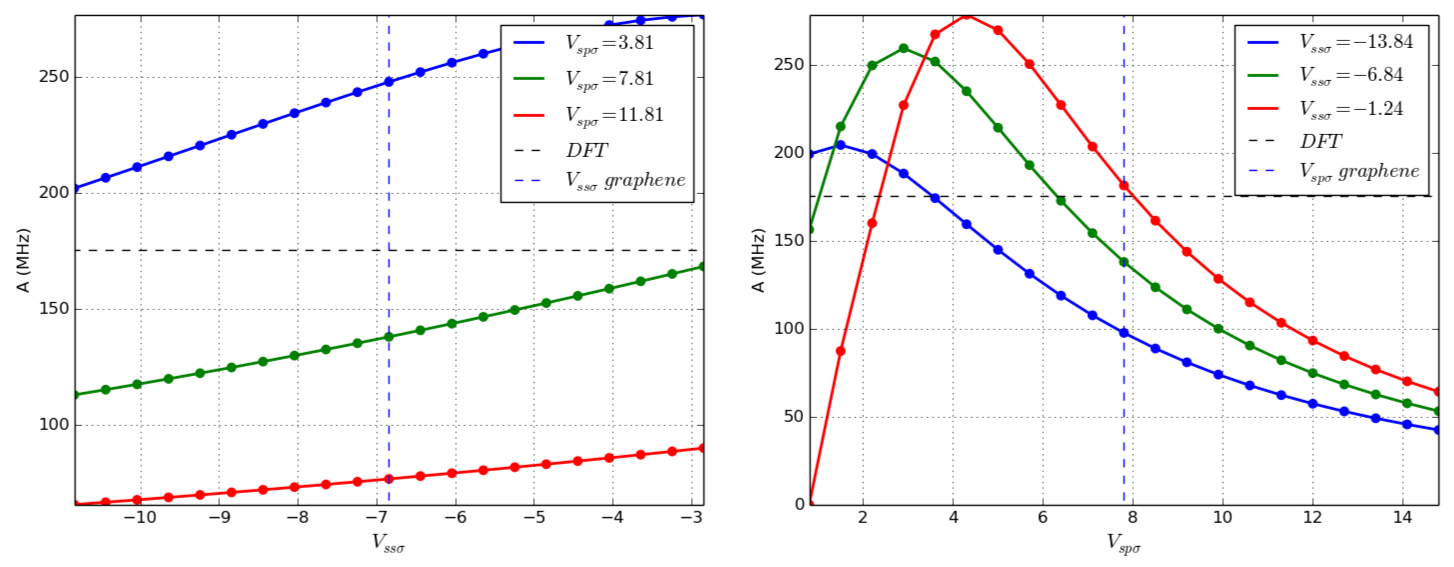
\includegraphics{chapter05/figures/hf_SK.png}
\vspace{-5pt}
\caption{Dependence of the hyperfine coupling $\mathcal{A}$ with the Slater-Koster parameters $V_{sp\sigma}$ and the $V_{ss\sigma}$.}
\label{hf_SK}
\end{figure}
\FloatBarrier
%~~~~~~~~~~~~~~~~~~~~~~~~~~~~~~~~~~~~~~~~~~~~~~~~~~~~~~~~~~~%
We can see a stronger dependence on the $Vsp\sigma$ as expected, and it is interesting to notice that in the (non-physical) limit of $Vsp\sigma\rightarrow0$ the hyperfine coupling decreases, this makes sense since reducing this coupling means isolating the Hydrogen, hence the effective hyperfine coupling of the ``zero-energy'' state would not have any component on the $s$ orbital of the Hydrogen.

The Slater-Koster parameters are fitted to achieve better agreement in the hyperfine coupling.

Since \ac{tb} and \ac{dft} seem to be compatible, we restrict the calculations of bigger islands only to TB so we can avoid the enormous computational cost of \ac{dft} for large systems.\\

As depicted in figure \ref{hyper} we can see that the effective hyperfine coupling decreases as the islands get bigger. The reason for this behavior is strongly related to the change in the gap in the spectrum. The larger the island is, the smaller the confinement gap gets.
%~~~~~~~~~~~~~~~~~~~~~~~~~~ FIGURE ~~~~~~~~~~~~~~~~~~~~~~~~~%
\begin{figure}
\centering
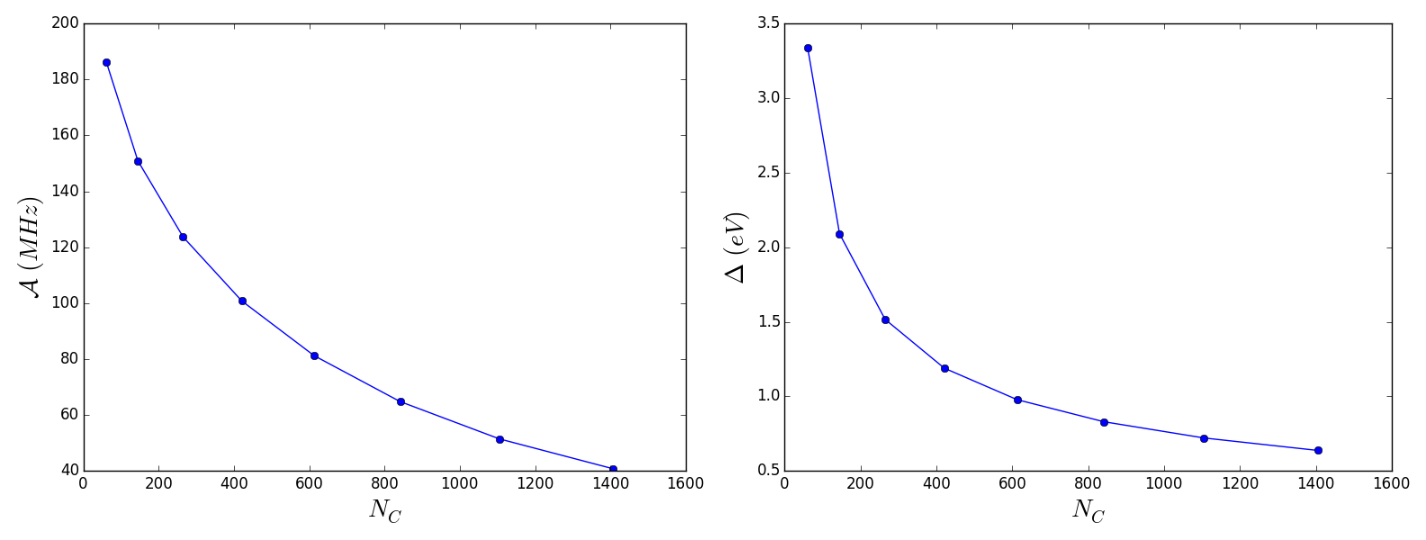
\includegraphics[width=0.9\textwidth]{chapter05/figures/hypergap.png}
\caption{$a)$ Effective hyperfine interaction dependence with the number of atoms (proportional to the island size). $b)$ Gap as a function of the island size}
\label{hyper}
\end{figure}
\FloatBarrier
%~~~~~~~~~~~~~~~~~~~~~~~~~~~~~~~~~~~~~~~~~~~~~~~~~~~~~~~~~~~%




\red{WTF ------}

When we plot this dependence of the hyperfine coupling with the gap, we find
%~~~~~~~~~~~~~~~~~~~~~~~~~~ FIGURE ~~~~~~~~~~~~~~~~~~~~~~~~~%
\begin{figure}[h!]
\centering
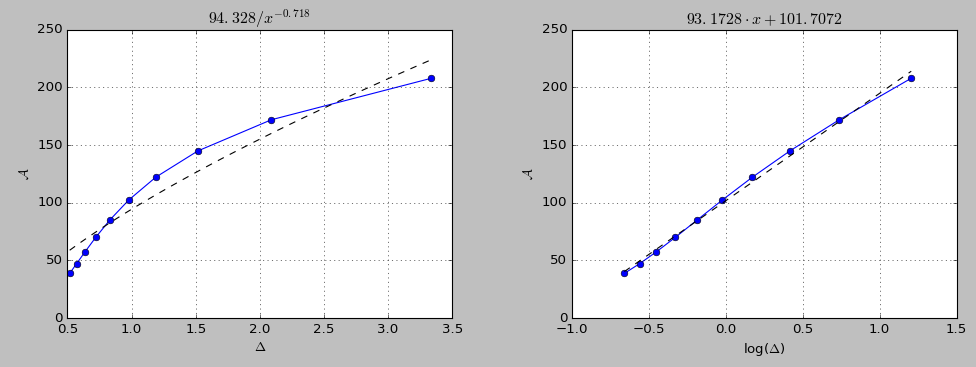
\includegraphics[width=0.9\textwidth]{chapter05/figures/A_gap.png}
\vspace{-5pt}
\caption{Dependence of the hyperfine coupling with the gap.}
\end{figure}
\FloatBarrier
%~~~~~~~~~~~~~~~~~~~~~~~~~~~~~~~~~~~~~~~~~~~~~~~~~~~~~~~~~~~%
I don't understand this dependence.

\red{WTF ------}






The relation between the hyperfine coupling and the gap arises from the dependence of the extension of the \blue{zero energy} wave function on the size of the gap. This dependence can be quantified by calculating the inverse participation ratio (ipr)
\begin{equation}
  \text{ipr} = \eta = \displaystyle\sum_{\alpha}|\psi_{0}(\alpha)|^4
\end{equation}
where $\alpha$ labels all the atoms \blue{(orbitals)} in the unit cell, and the subindex $0$ specifies the zero energy state. Note that for a evenly completely delocalized state it is expected that $\eta\rightarrow1/N$ while for a state mostly localized in one atom $\eta\rightarrow1$. In our case, from Lieb's theorem we expect that our midgap state would be sublattice polarized (hence localized only in $N/2$ atoms), so if the state were to be evenly distributed in half of the atoms in the island the ipr would be $\eta\rightarrow2/N$. Surprisingly this prediction is quite accurate as can be seen in figure \ref{ipr}.
%~~~~~~~~~~~~~~~~~~~~~~~~~~ FIGURE ~~~~~~~~~~~~~~~~~~~~~~~~~%
\begin{figure}
\centering
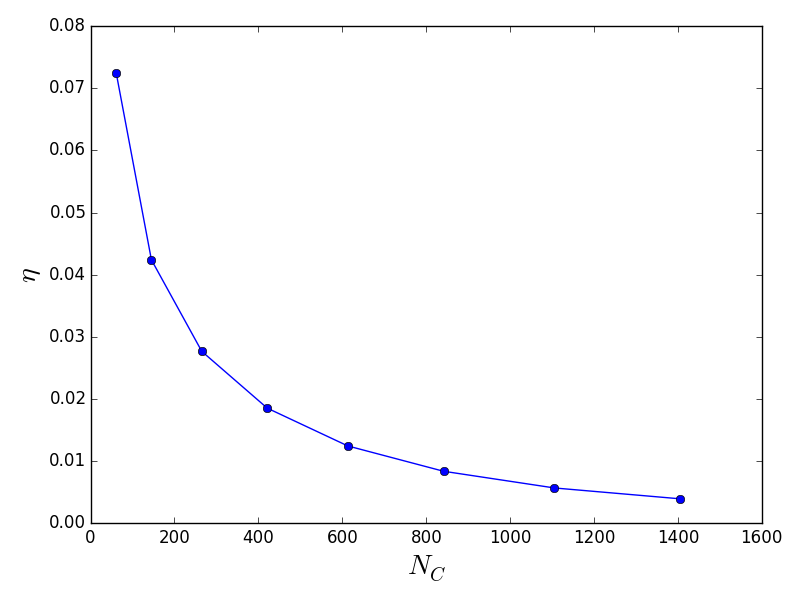
\includegraphics[width=0.5\textwidth]{chapter05/figures/ipr.png}
\caption{\red{(missing fit in the plot, but it'll be there)} ipr, $\eta$ as a function of the island size. The dashed line corresponds to the expected dependence, for larger islands this prediction gets more accurate.}
\label{ipr}
\end{figure}
\FloatBarrier
%~~~~~~~~~~~~~~~~~~~~~~~~~~~~~~~~~~~~~~~~~~~~~~~~~~~~~~~~~~~%
It seems paradoxical that knowing that the vast majority of the wave function is located in the 3-6 closest neighbors (see figure \ref{spectrum1}) the ipr looks so similar to the evenly distributed case.

\blue{testing}

To clarify how is the actual localization of this state we will plot the weight of the wave function in each atom versus the distance to the vacancy.
%~~~~~~~~~~~~~~~~~~~~~~~~~~ FIGURE ~~~~~~~~~~~~~~~~~~~~~~~~~%
\begin{figure}[h!]
\centering
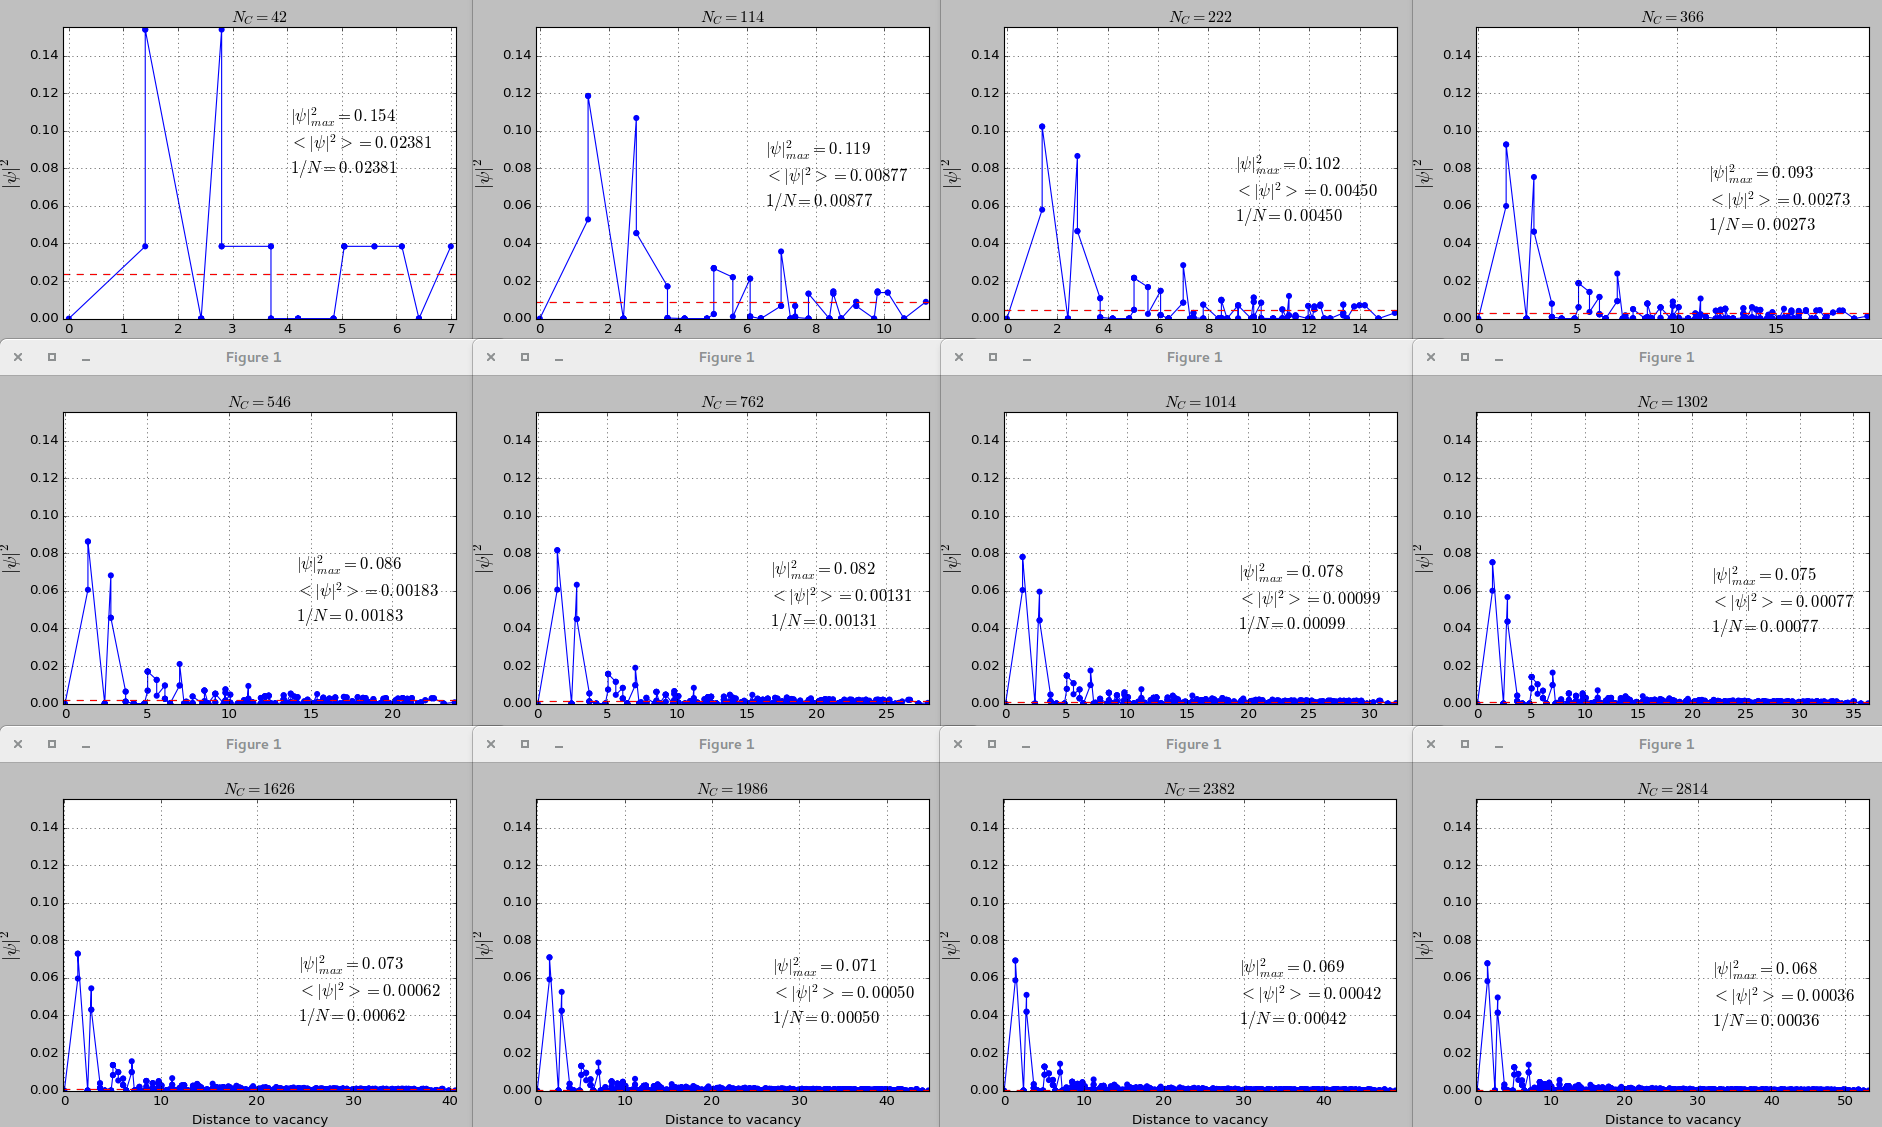
\includegraphics[width=1\textwidth]{chapter05/figures/spatial_distribution.png}
\vspace{-5pt}
\caption{Spatial distribution for different sizes of the unit cell for armchair islands.}
\end{figure}
\FloatBarrier
%~~~~~~~~~~~~~~~~~~~~~~~~~~~~~~~~~~~~~~~~~~~~~~~~~~~~~~~~~~~%
The interesting part is that for all the islands it follows that
\begin{equation}
  \mean{|\psi|^2} = \frac{1}{N}
\end{equation}

Also, the ipr for an evenly localized states is
\begin{equation}
  \eta = \frac{1}{N}
\end{equation}




\red{RAW}

The magnetic state associated to a vacancy in graphene is a completely delocalized state, hence $\eta\rightarrow1/N$, yet its spatial profile is not that of an evenly distributed state. Instead it keeps some fraction


Magnetism of the first neighbor
%~~~~~~~~~~~~~~~~~~~~~~~~~~ FIGURE ~~~~~~~~~~~~~~~~~~~~~~~~~%
\begin{figure}[h!]
\centering
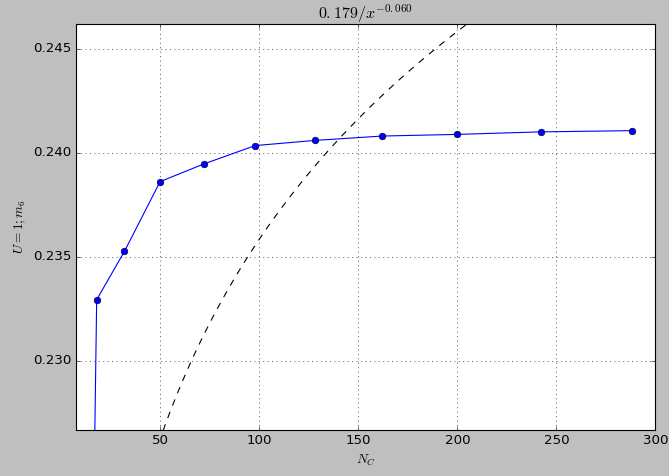
\includegraphics{chapter05/figures/mag_6neig.png}
\vspace{-5pt}
\caption{magnetic moment of the six nearest atoms in a MF Hubbard calculation with embedding}
\end{figure}
\FloatBarrier
%~~~~~~~~~~~~~~~~~~~~~~~~~~~~~~~~~~~~~~~~~~~~~~~~~~~~~~~~~~~%




%~~~~~~~~~~~~~~~~~~~~~~~~~~ FIGURE ~~~~~~~~~~~~~~~~~~~~~~~~~%
\begin{figure}[h!]
\centering
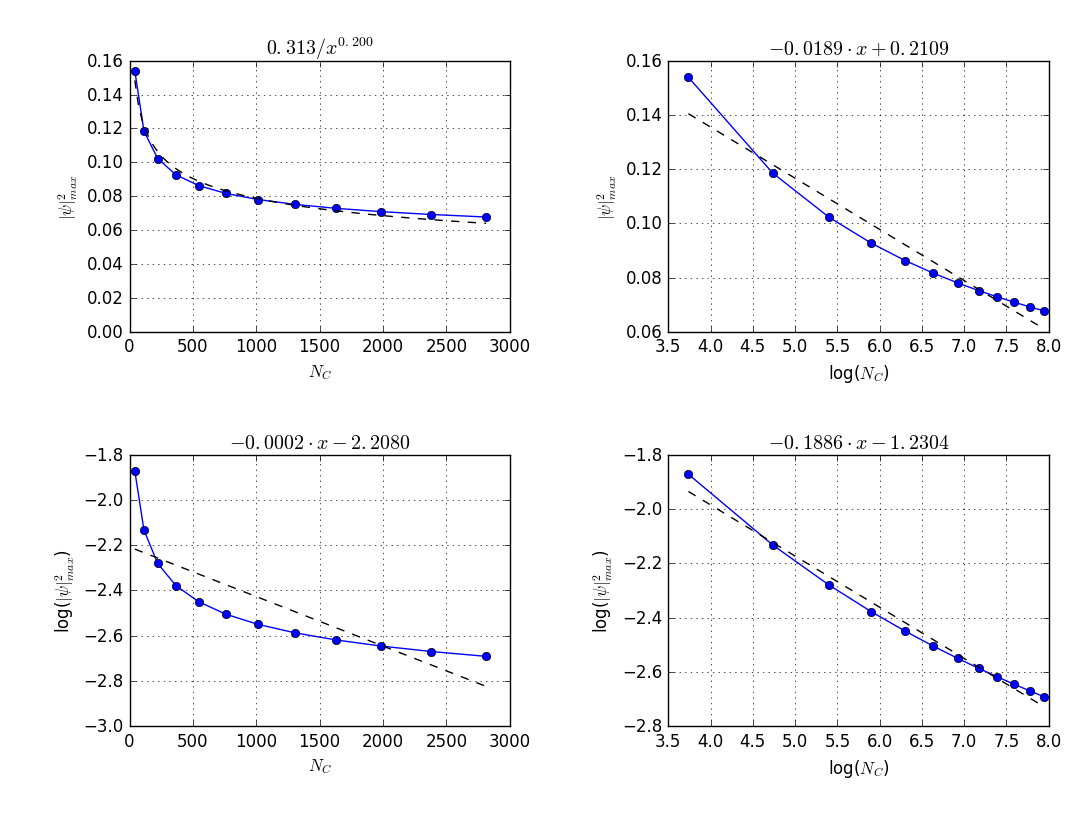
\includegraphics{chapter05/figures/maxfunc_Nc.png}
\vspace{-5pt}
\caption{$|\psi|^2_{max}$ as a function of the size of the island}
\end{figure}
\FloatBarrier
%~~~~~~~~~~~~~~~~~~~~~~~~~~~~~~~~~~~~~~~~~~~~~~~~~~~~~~~~~~~%





\section{Periodic systems}
Because I have done the calculations already
\subsection{1D}
Just ribbons
%~~~~~~~~~~~~~~~~~~~~~~~~~~ FIGURE ~~~~~~~~~~~~~~~~~~~~~~~~~%
\begin{figure}[h!]
  \centering
  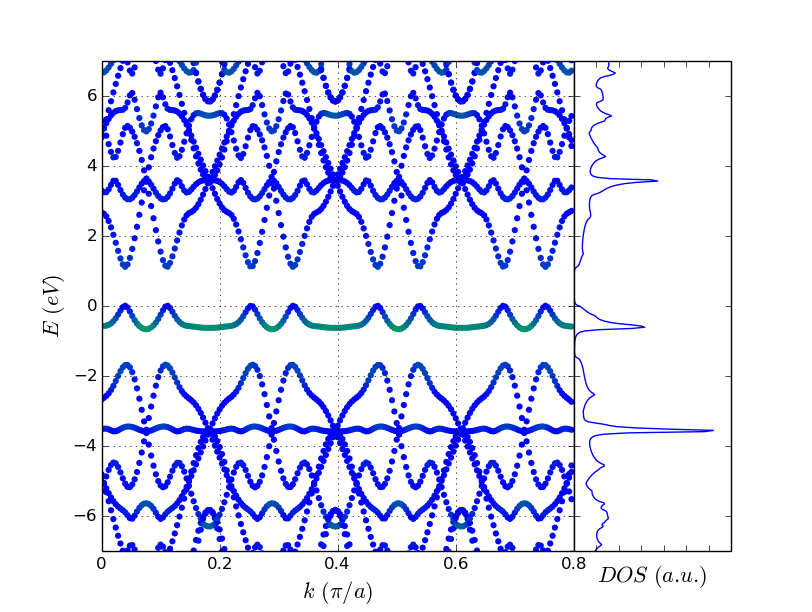
\includegraphics{chapter05/figures/2dbands.png}
  \vspace{-5pt}
  \caption{Band strcuture for a graphene nanoribbon with a periodic array of hydrogen adatoms}
\end{figure}
\FloatBarrier
%~~~~~~~~~~~~~~~~~~~~~~~~~~~~~~~~~~~~~~~~~~~~~~~~~~~~~~~~~~~%
\subsection{2D}
periodic array.




\section{Single vacancy limit}
As we have seen, the limit of a single vacancy is quite complicated since graphene presents zero \ac{dos} at the Fermi energy (like an insulator) yet it has a finite \ac{dos} at infinitesimally close energies (like a metal). In any case, either if we consider a 0-D system, or a periodic defected unit cell, the system will always present a gap\footnote{for some specific geometries this is not exactly true, but any interaction will open a gap, so the zero energy states present in these cases are not robust at all.}, and will not in fact be the proper model for one single adatom in graphene.\\
If we want to address the problem of \textbf{a single defect in infinite pristine graphene} we need a different set of tools.

\subsection{Embedding technique}
If we try to describe a single defect in an otherwise infinite and pristine system using the previous \ac{tb} description we would need to expand our basis and consider all the possible sites. For a truly infinite system, where no two atoms are equivalent, we would actually need an inifinite basis.
Since the translational symmetry of the system is broken, the Bloch's theorem no longer applies and a new set of tools is needed.

We will describe the system using the Green's function formalism. We start by splitting the complete (infinite) system in two regions, a defected area (a finite cell\footnote{Not a cell in the sense of a periodic unit cell, but rather just a few atoms in which to study the properties we are interested in.} containing one or more defects) and the rest of the infinite system as shown in Fig.~\ref{DOS}~(b). This division will allow the calculation of the self-energy due to the coupling between regions.

We will start by considering a completely pristine crystal with translational symmetry. Such a system can be split in two regions (Fig.~\ref{DOS}~(b)), the unit cell, region $A$ and everything else, region $B$.
With this distribution of the system, the Hamiltonian of the whole (infinite) system can be written as
\begin{equation}
  H = \left(\begin{array}{cc}
     H_{A} & V_{AB} \\
     V_{BA} & H_{B}
   \end{array}\right) =
  \left(\begin{array}{cc}
   H_{A} &  0  \\
    0     & H_{B}
  \end{array}\right)+
  \left(\begin{array}{cc}
    0 & V_{AB} \\
   V_{BA} & 0
  \end{array}\right)
\end{equation}
When a Hamiltonian has this structure, the Green's function corresponding to the region $A$ can be written (exactly) using the Dyson equation.
\begin{equation}
  G_{A} = \frac{1}{E-H_{A}-V_{AB}\frac{1}{E-H_{B}}V_{BA}}
\end{equation}

Usually this equation is understood as a renormalization of the Hamiltonian for region $A$ by its interaction with the rest of the system ($V_{AB}$). This renormalization yields an effective Hamiltonian:
\begin{equation}
  H'_{A} = H_{A}+V_{AB}\frac{1}{E-H_{B}}V_{BA} = H_{A} + \Sigma_{AB}
\end{equation}

Naively we could think that from this formula we could calculate the self-energy $\Sigma_{AB}$, but we have to remember that the region B corresponds to an infinite crystal, so the Hamiltonian $H_{B}$ would have infinite dimension, and since it does not have translation symmetry (on account of the hollow due to region $A$) its calculation is impossible.

Nevertheless even if we cannot calculate yet $\Sigma_{AB}$ it is still true that the Green's function for the region $A$ can be exactly expressed as:
\begin{equation}
G_{A}(E) = \frac{1}{E - H_{A}-\Sigma_{AB}}
\label{Gdyson}
\end{equation}

The calculation of the self-energy $\Sigma_{AB}$ is made possible considering two facts. First, we have to notice that all the information of the coupling between the regions $A$ and $B$ is encoded in the self-energy $\Sigma_{AB}$, which will not depend on the content of $A$ but rather on its conectivity to $B$. Second, the equation \eqref{Gdyson} holds true for the pristine case in which the translation symmetry allows a Bloch calculation of $G_A$.
%
% For the particular case of a periodic system (with translational symmetry) there is an easy way of calculating this self-energy $\Sigma_{AB}$.
%
% If the system does have translational symmetry, there is nothing that differentiates the regions $A$ and $B$  (other than our will). A Bloch's description of the system is in this case allowed, and therefore the Green's function for the $A$ region (now considered as an unit cell) can be calculated by integrating the $\vec{k}$ dependent Green's function over the whole Brillouin zone.
\begin{equation}
G_{A}(E) = \int_{FBZ}\frac{1}{E-H(\vec{k})}d\vec{k}
\label{Gbloch}
\end{equation}

Since we have two ways of calculating the same object (only for the pristine case), we can equate equations \eqref{Gdyson} and \eqref{Gbloch}, to get an expression for the self-energy
\begin{equation}
\Sigma_{AB} = E - H_{A} -\left(\int_{FBZ}\frac{1}{E-H(\vec{k})}d\vec{k}\right)^{-1}
\label{self-energy}
\end{equation}

Using equation \eqref{self-energy} we can calculate the self-energy that describes the effect of the coupling of the region $A$ to the region $B$.\\

Once $\Sigma_{AB}$ has been calculated (using the prisinte Hamiltonian), if the hopping to the rest of the system does not change because of the defect(s), we can calculate the Green's function for a defected $A$ region coupled to the pristine $B$ region as:

\begin{equation}
\widetilde{G}_A(E) = \frac{1}{E-\widetilde{H}_{A}-\Sigma_{AB}}
\label{green}
\end{equation}

Using this procedure we can calculate the Green's function of a defected unit cell coupled to a pristine crystal.
For the sake of notation we will drop the tilde and specify, when needed if the hamiltonian $H_A$ corresponds to a pristine or a defected one.\\


Equipped with this tool we proceed now to study the physical properties of a single defect on a pristine environment. We will describe graphene as a honeycomb lattice with only one orbital per site as justified in section~\ref{ch:graphene}. A hydrogen adatom in this framework appears as the effective removal of one of the sites in the lattice.

Using equations \eqref{self-energy} and \eqref{green} we calculate the \ac{dos} of an infinite sheet of graphene with a single vacancy. The \ac{ldos} can be calculated as
\begin{equation}
\rho_{i}(E) = -\frac{1}{\pi}\Im{G_{i,i}(E)} \quad\quad;\quad\quad
\rho(E) = -\frac{1}{\pi}\Im{Tr\left(G(E)\right)}
\label{eq:DOS}
\end{equation}
where $i$ labels any given atom. For the total \ac{dos} we just need to sum the contribution from all the atoms. For the sake of notation the trace will be dropped and only added for the final formulas, so unless there is an index specifying the site, the trace will be considered implicit in the formula.

%~~~~~~~~~~~~~~~~~~~~~~~~~~ FIGURE ~~~~~~~~~~~~~~~~~~~~~~~~~%
\begin{figure}[h!]
\centering
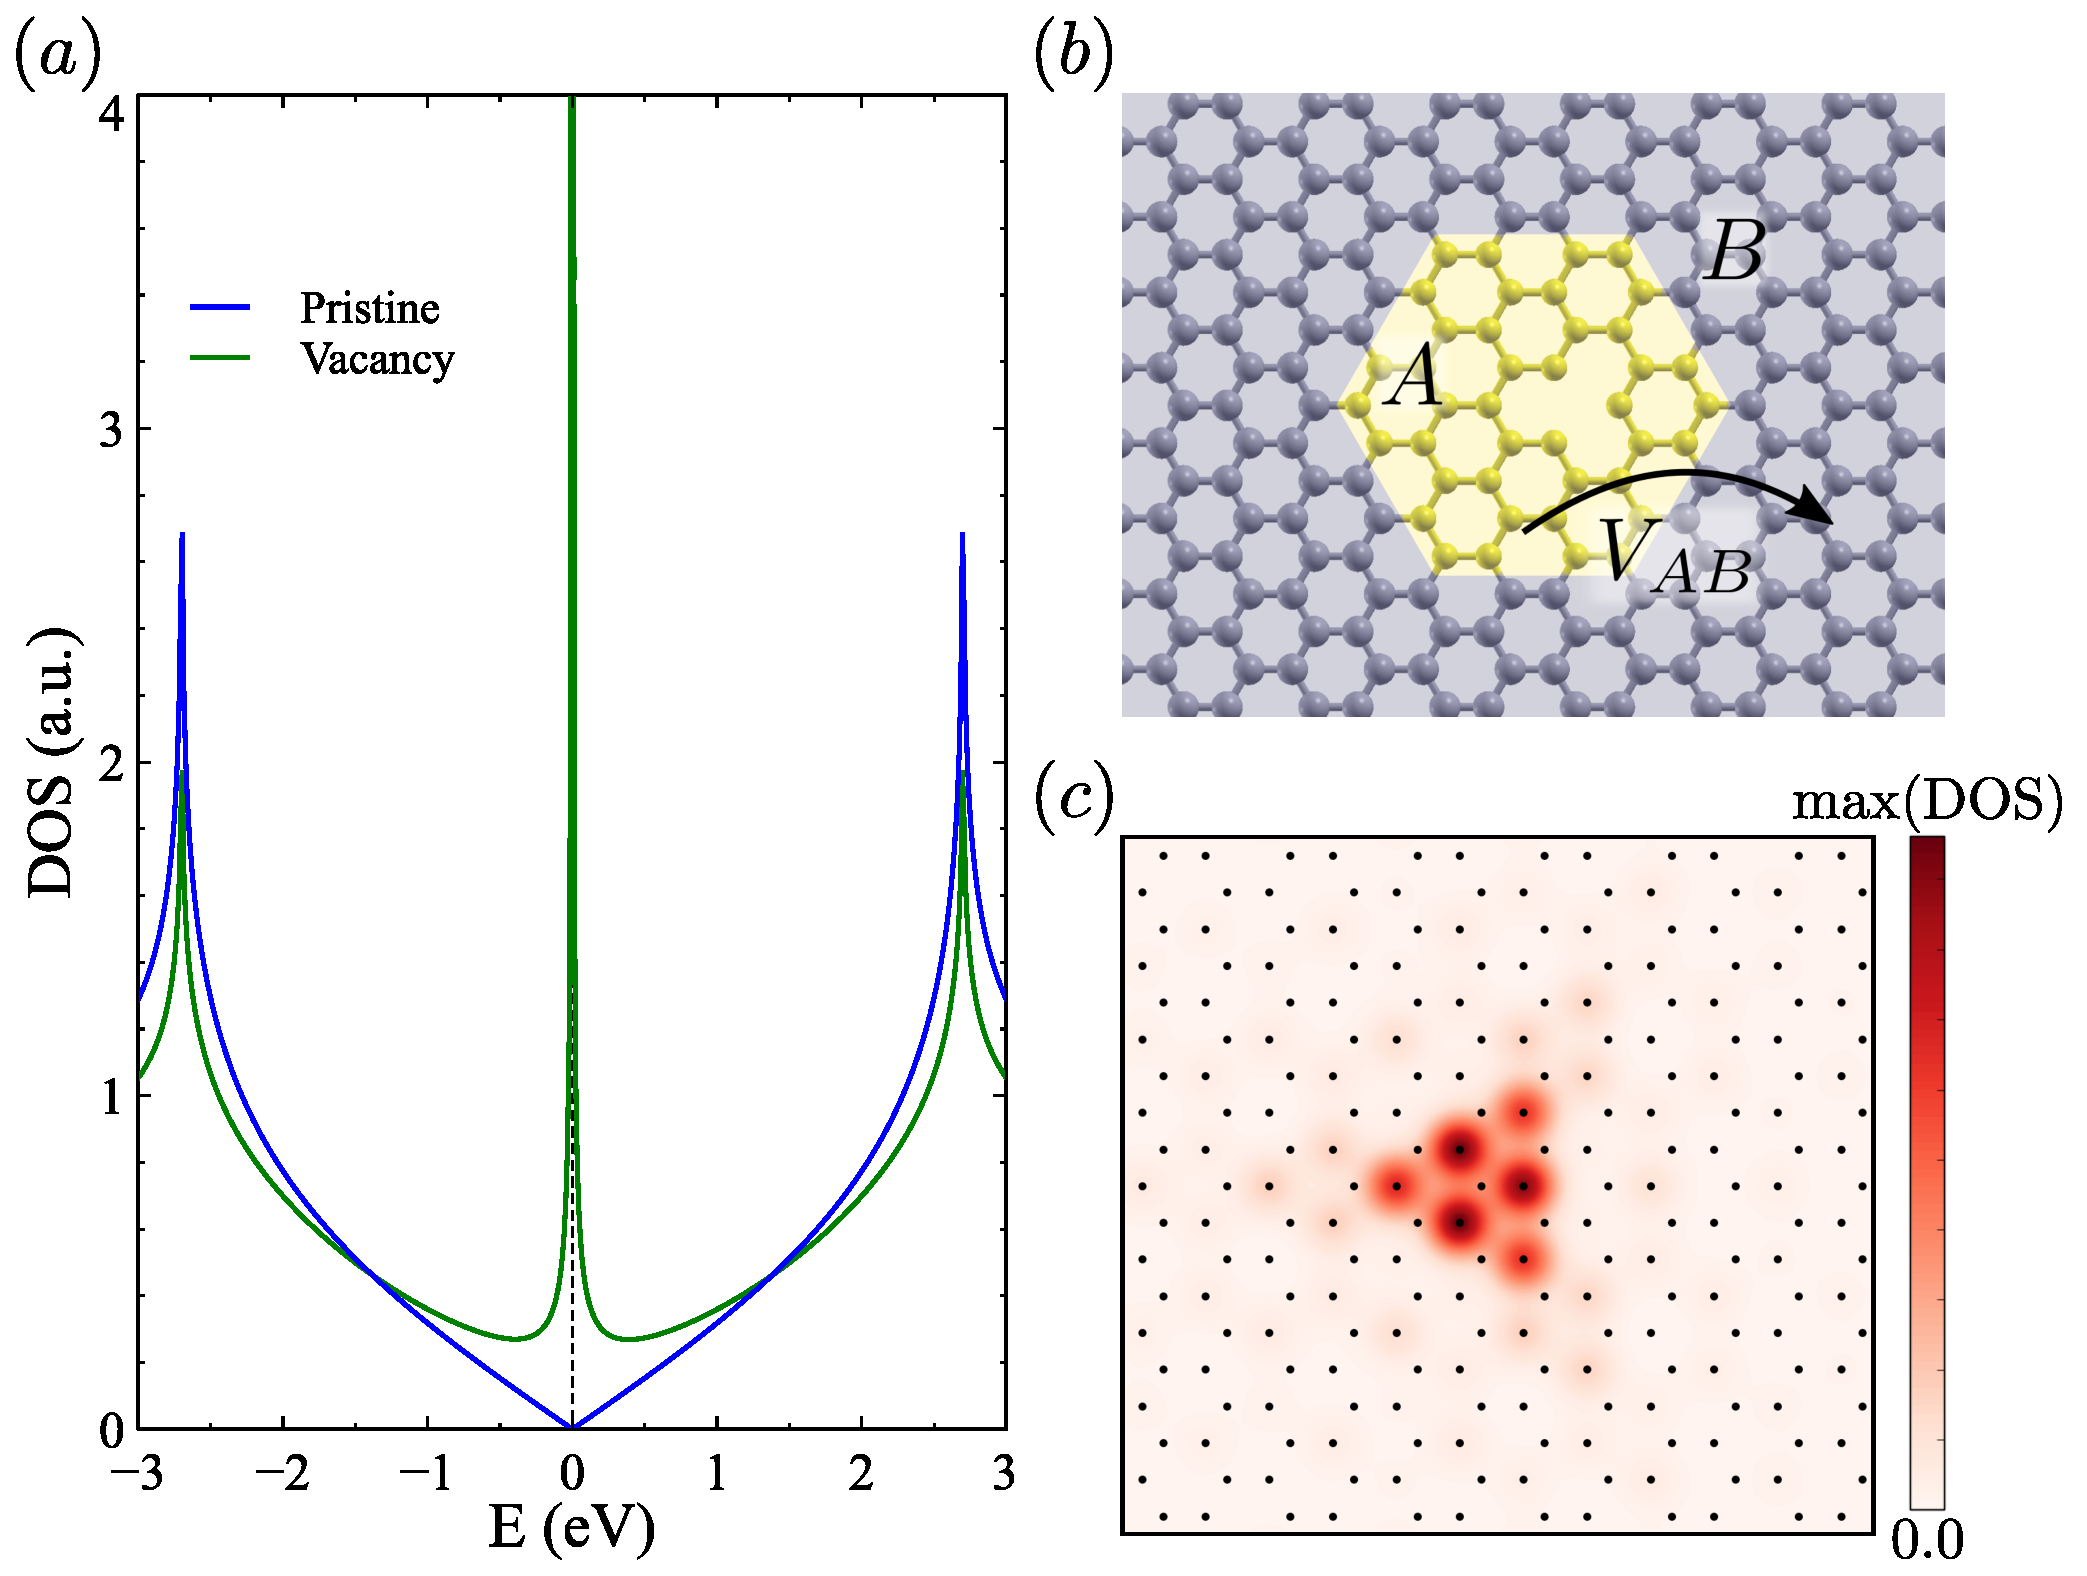
\includegraphics{chapter05/figures/DOSlDOS.pdf}
\vspace{-5pt}
\caption{$a)$ Total \ac{dos} of a single vacancy in an infinite graphene sheet. A divergence in the \ac{dos} appears at $E=0$ when the vacancy is introduced. $b)$ \ac{ldos} for the zero energy state related to a vacancy in graphene. Side by side we can compare the calculations for two unit cells with different size. The vacancy is depicted as a white circle. As expected the (real) spatial distribution of this state is located in the 3-6 closest atoms to the vacancy (of one sublattice).}
\label{DOS}
\vspace{-5pt}
\end{figure}
%~~~~~~~~~~~~~~~~~~~~~~~~~~~~~~~~~~~~~~~~~~~~~~~~~~~~~~~~~~~%

The result of the introduction of a single vacancy can be seen in Fig.~\ref{DOS}~(a). A resonance appears at energy $E=0$ getting some spectral weight from higher energy states.
It is interesting to study the spatial distribution of this zero energy resonance, Fig.~\ref{DOS}~(c), as described in previous work, the main contribution for this state comes from the 3-6 nearest neighbors to the vacancy belonging to a different sublattice from that of the missing site.\\

Notice that the calculation inside the region $A$ is exact, yet this does not mean that the description of the zero energy state is complete. Since we are matching a unit cell to a pristine system we are imposing that in region $B$ the system is pristine graphene, so we will not be able to capture the whole state, but the part that we do capture, will be exact.
This means that we need to be careful in the analysis not to include effects related just to the size of the unit cell and study all the properties as a function of the size of the unit cell.




\subsection{Non interacting temperature magnetization}
To study the magnetic properties the system we proceed to apply an external in-plane magnetic field to the system, and calculate its magnetic response. The Zeeman term for an electron takes the form
\begin{equation}
  H^{Zee} \propto B\sigma^e_{z}
\label{zee}
\end{equation}
The effect of such a term is expected to rigidly shift to higher energies the spin up channel while lowering the energies of the spin down channel (see Fig.~\ref{magnetization}~(a)).

To calculate the magnetization we just need to compute the difference in the \ac{dos} of the spin up and down. The \ac{dos} is calculated using \eqref{eq:DOS}, then integrating the Green's function up to the Fermi Energy and taking the imaginary part.
\begin{equation}
  m = \frac{-1}{\pi}
      \Im{\int^{0}_{-\infty} (G^{\uaw}(E)-G^{\daw}(E))dE}
\end{equation}
Nevertheless since the Zeeman term \eqref{zee} shifts symmetrically the up and down spin channels the following relations are true
\begin{equation}
  G^{\uaw}(E) = G(E-B) \quad\quad;\quad\quad G^{\daw}(E) = G(E+B)
\end{equation}
where $G$ refers to the spinless Green's function. The magnetization then can be rewritten as follows:
\begin{equation}
  \begin{split}
      m = \frac{-1}{\pi}\Im{\int^{0}_{-\infty}(G(E+B)-G(E -B))dE} =\\
      \frac{-1}{\pi} \Im{\Tr{\int^{B}_{-B}G(E)dE}}
  \end{split}
\label{mmag}
\end{equation}
Notice that we only need to calculate the spinless Green's function to calculate the magnetization of the system.

We will consider only the magnetization of the 3 nearest atoms since otherwise as the cell grows larger, the magnetism of the atoms far away from the defect would overcome the contribution of the ``perturbed ones'' making it difficult to see the actual effect of the defect. The equation \eqref{mmag}, hence, gets reduced to:
\begin{equation}
  m = -\frac{1}{\pi}
      \Im{\sum^{3}_{i}\int^{B/2}_{-B/2}G_{i,i}(E)dE}
\label{mag}
\end{equation}
where the index $i$ labels the 3 atoms closest to the vacancy.

%~~~~~~~~~~~~~~~~~~~~~~~~~~ FIGURE ~~~~~~~~~~~~~~~~~~~~~~~~~%
\begin{figure}[h!]
\centering
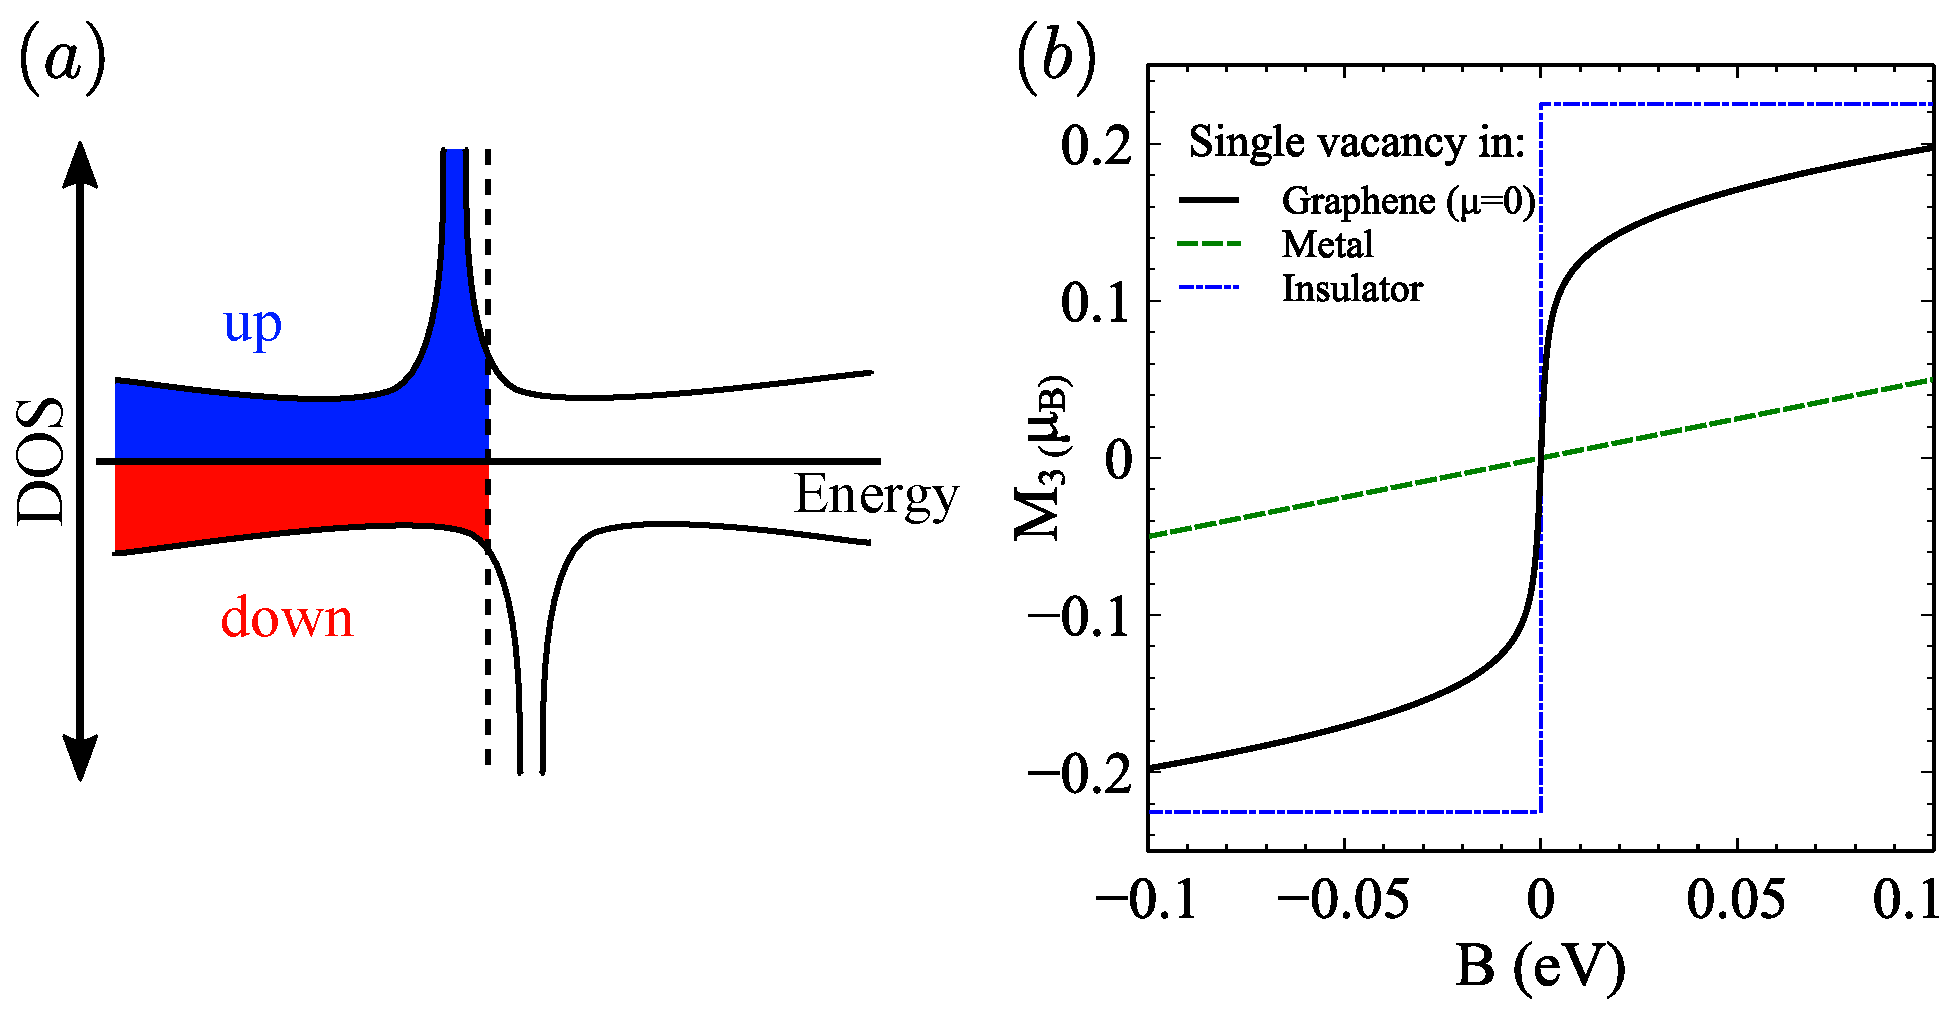
\includegraphics{chapter05/figures/comparison.pdf}
\vspace{-5pt}
\caption{$(a)$ Sketch of the DOS (per spin flavor) of an impurity in the presence of an external magnetic field coupled only via Zeeman effect. $(b)$ magnetization of the first 3 neighbors of the defect as a function of the applied magnetic field for a hydrogen atom in a graphene quantum dot (blue) and a single hydrogen atom in pristine graphene (black), the green line is the result for a conventional metal, modeled by graphene with the chemical potential well above the Dirac point.}
\label{magnetization}
\end{figure}
%\FloatBarrier
%~~~~~~~~~~~~~~~~~~~~~~~~~~~~~~~~~~~~~~~~~~~~~~~~~~~~~~~~~~~%

As we can see in Fig.~\ref{magnetization}~(b) the magnetization of this system is not that of a regular metal, nor that of a typical paramagnet. In this case, for infinitesimally small magnetic fields the magnetic response (the slope of the function drawn in \ref{magnetization}) gets arbitrarily big. This divergence in the magnetic response is a sign of a magnetic instability that motivates further study.




\subsection{Finite temperature susceptibility}
Since the magnetic behavior of a vacancy in graphene is not that of a metal, nor that of a well-defined state in a gap, its behavior with the temperature may change as well.

The main modification in the formalism when considering the temperature dependence is the introduction of the Fermi-Dirac distribution function in the integrals of the Green's function (for the \ac{dos} and magnetic moment).

The integral in the calculation of the total magnetic moment in the presence of an in-plane magnetic field $B$ now reads
\begin{equation}
  m=\int^{\infty}_{-\infty} \left[G^{\uaw}(E)-G^{\daw}(E)\right]n_{f}(E,T)dE
\end{equation}
Or, equivalently, in terms of the spinless Green's function
\begin{equation}
  m=\int^{\infty}_{-\infty} \left[G(E-B)-G(E+B)\right]n_{f}(E,T)dE
\end{equation}
By using a change of variables like $E\pm B\rightarrow E'$ we can rewrite the magnerization as:
% \begin{equation}
%   m(T) = \int^{\infty}_{-\infty} G(E')n_{f}(E-B,T)dE' -
%   \int^{\infty}_{-\infty} G(E')n_{f}(E+B,T)dE'
% \label{magT}
% \end{equation}
\begin{equation}
  m(B,T) = \frac{-1}{\pi}\Im{Tr\left(
  \int^{\infty}_{-\infty} G(E)\left[n_{f}(E-B,T)-n_{f}(E+B,T)\right]dE\right)}
\label{magT}
\end{equation}

% Notice that if we want to calculate this integral using the residue theorem now we have to take into account the poles of the Fermi's distribution function:
% \begin{equation}
%   n_{f}(E,T) = \frac{1}{1+e^{(E-\mu)/k_{B}T}}
%     \quad\Rightarrow\quad
%    E_{Poles} = i(2n-1)\pi k_{B}T+\mu
% \end{equation}
%
% % The calculation of the poles could be tricky, so let's do it explicitely. $G(E)$ presents poles only under the real axis, so it will not contribute to the poles. Calling $\delta=B/2$, and using that $\mu=0$ and $\beta=1/k_{B}T$
% %
% % \begin{equation}
% %   n_{f}(E'-\delta,T)-n_{f}(E'+\delta,T) =
% %   \frac{1}{1+e^{(E-\delta\beta)}} - \frac{1}{1+e^{(E+\delta\beta)}} =
% %   \frac{(1+e^{(E+\delta\beta)}-(1+e^{(E-\delta\beta)}))}{(1+e^{(E+\delta\beta)})(1+e^{(E-\delta\beta)})}
% % \end{equation}
% %
% % The poles will be given by the zeros of that denominator:
% % \begin{equation}
% %   \left(1+e^{(E+\delta\beta)}\right) \left(1+e^{(E-\delta\beta)}\right) = 0
% %   \quad\Rightarrow\quad
% %   e^{E\beta}\left(e^{\delta\beta}+e^{-\delta\beta}\right)+e^{2E\beta} = -1
% % \end{equation}
%
% This means that the integral \eqref{magT} can be calculated (calling the integrand $f(E)$)
% \begin{equation}
%   \int^{\infty}_{-\infty}f(E)dE =
%    -i2\pi\sum_{i_{Poles}}\text{Res}\left[f(E_{i_{Poles}})\right] +\int_{l}f(E)dE
% \end{equation}
% where $l$ is any path over the complex plane (with positive imaginary part) and the summation runs over all the poles enclosed by $l$.


%~~~~~~~~~~~~~~~~~~~~~~~~~~ FIGURE ~~~~~~~~~~~~~~~~~~~~~~~~~%
\begin{figure}[h!]
\centering
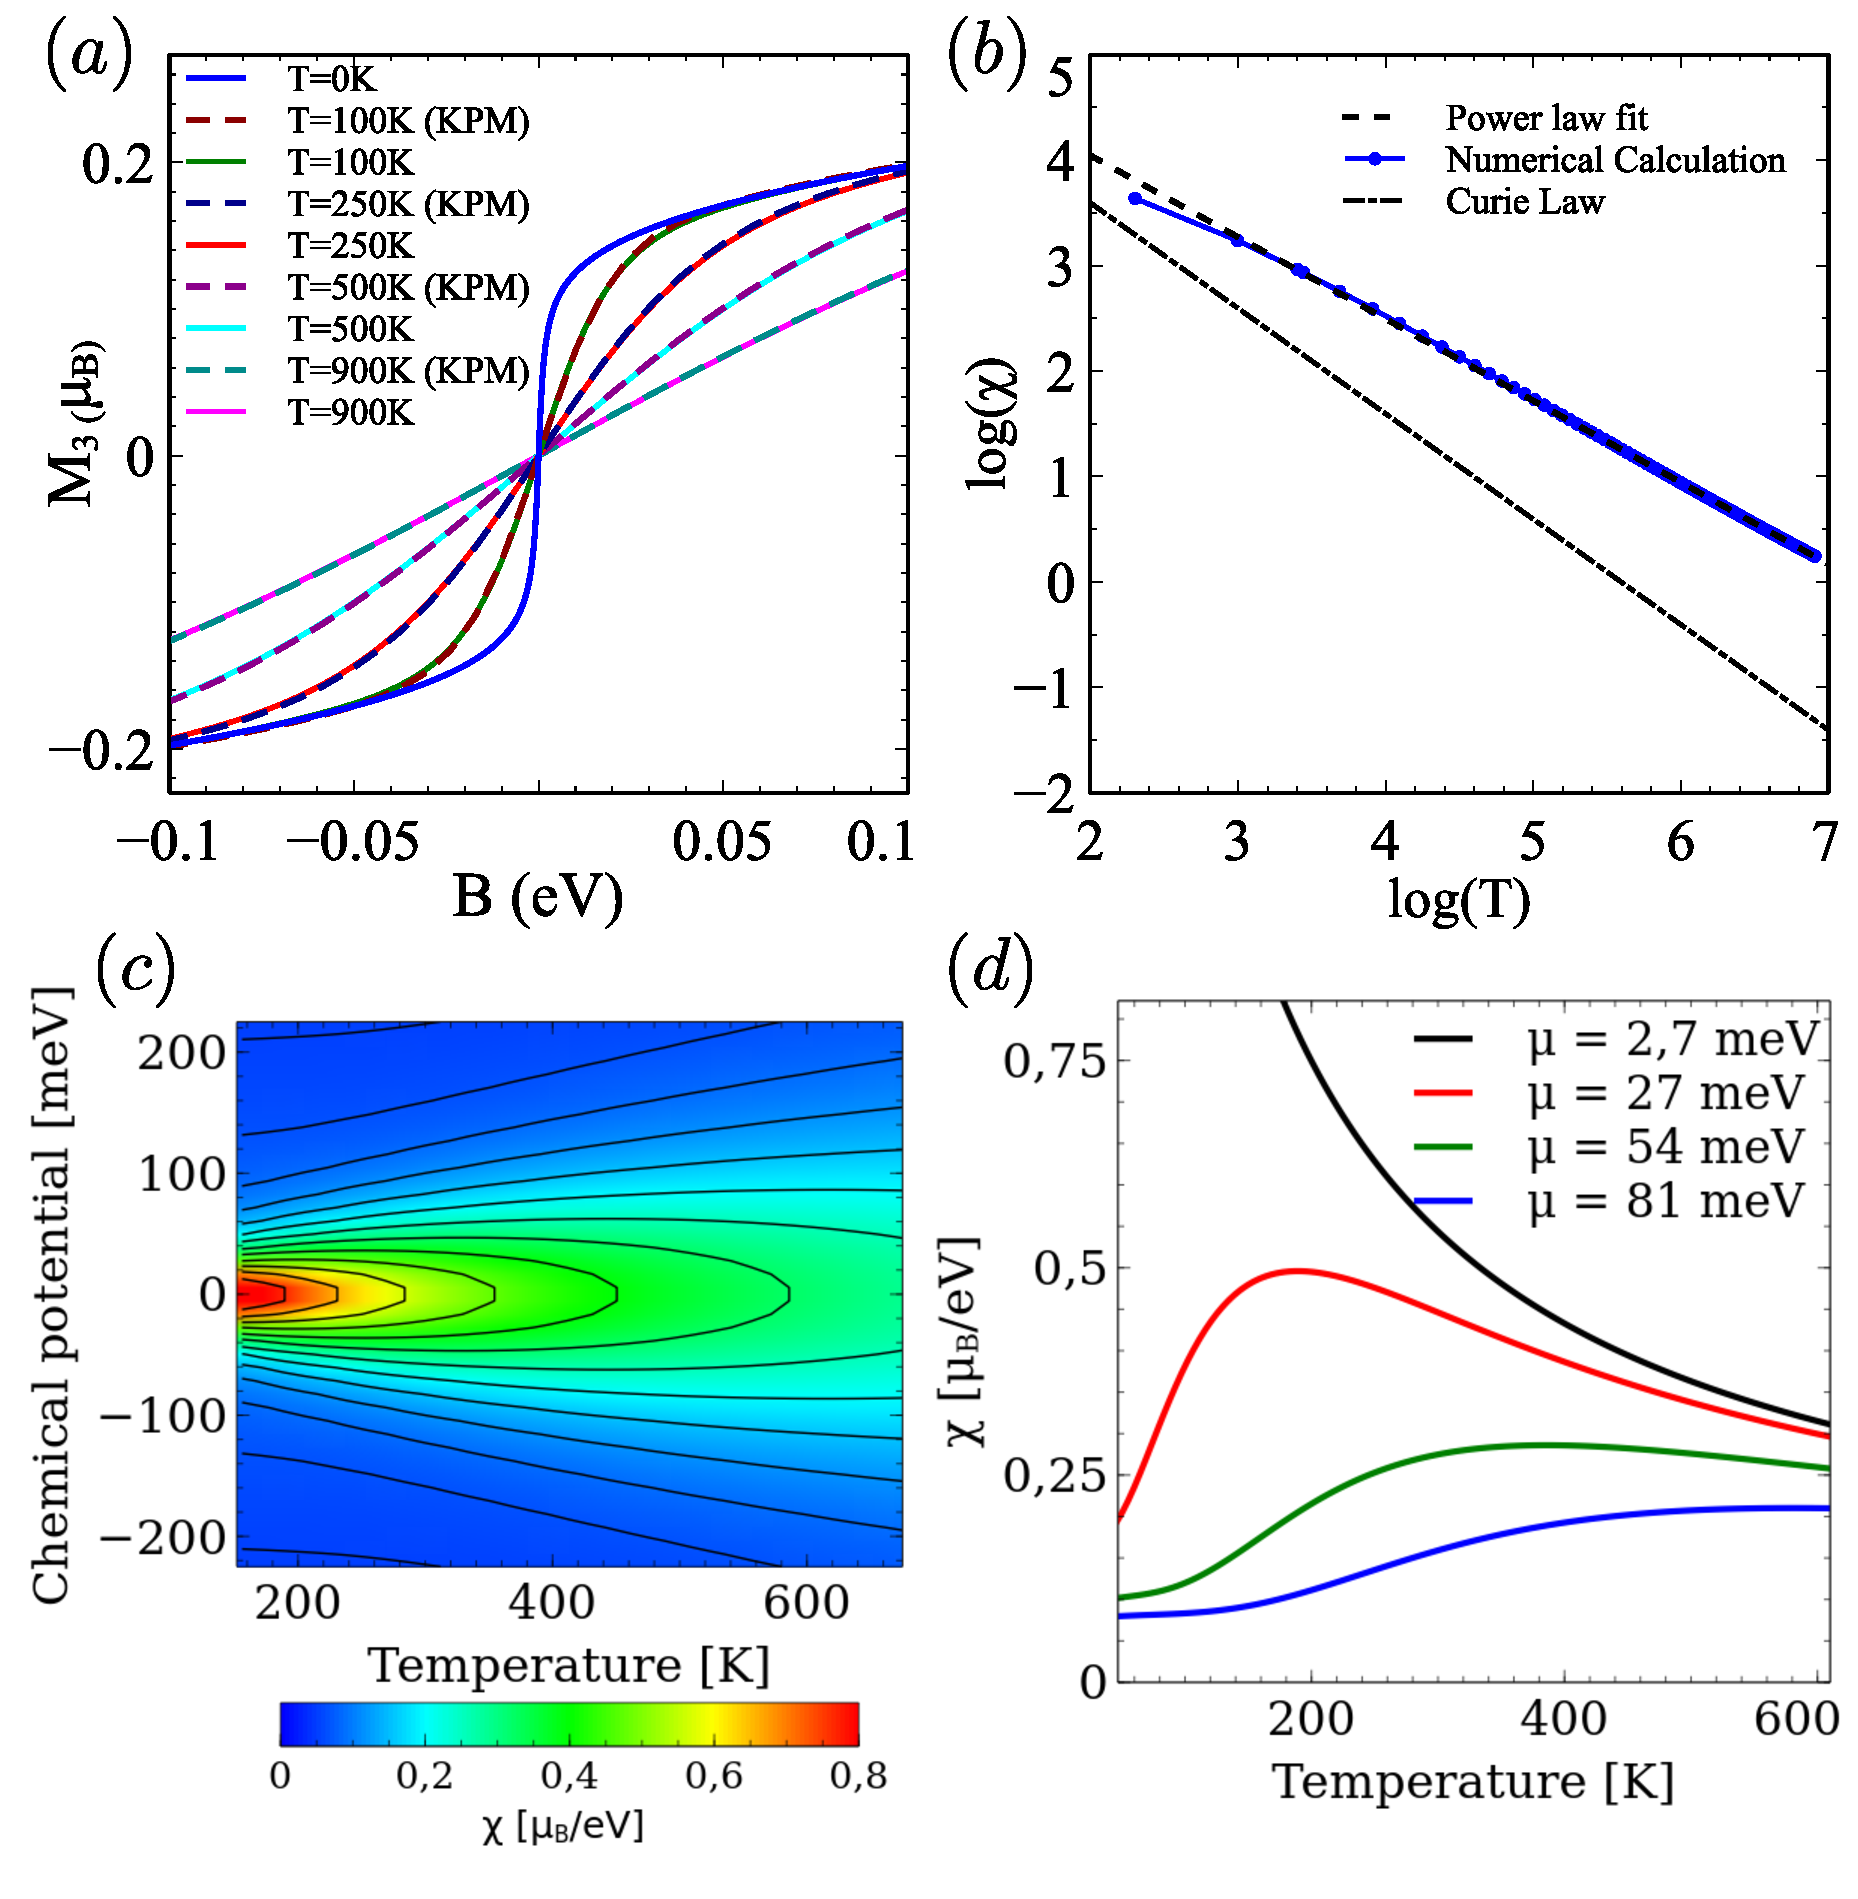
\includegraphics{chapter05/figures/temp_sus.pdf}
\vspace{-5pt}
\caption{$(a)$ Magnetization of the first 3 neighbors of the vacancy as a function of the applied magnetic field for different temperatures, dashed lines are calculated using the KPM and continuous lines are calculated using the embedding method.
$(b)$ Temperature dependence of the susceptibility in comparison with Curie’s Law. $(c-d)$ Dependence of the susceptibility with the doping and the temperature, showing that for some values of $\mu$ there is a non-monotonous behavior of the susceptibility with temperature.}
\label{temperature}
\end{figure}
\FloatBarrier
%~~~~~~~~~~~~~~~~~~~~~~~~~~~~~~~~~~~~~~~~~~~~~~~~~~~~~~~~~~~%
The main effect of the temperature in the magnetization is to smooth out the magnetic response of the system as shown in Fig.~\ref{temperature}~(a).

The susceptibility is defined as the derivative of the magnetization in the limit where $B\rightarrow0$
\begin{equation}
  \chi(T) = \left.\frac{\partial m(B,T)}{\partial B}\right|_{B\rightarrow0}
\end{equation}
and its dependence with the temperature is shown in Fig.~\ref{temperature}~(b).
The calculations are shown in a log-log plot to stress the power-law dependence.

For a conventional local magnetic moment, the zero field susceptibility follows the Curie law $\chi(T)\propto T^{-1}$. This result holds true, based on very general considerations, for any spin governed by the Hamilltonian \eqref{zee}.
In paricular the Curie susceptibility of a single electron in an in-gap level will follow a Curie law. Numerical derivation of the results of Fig.~\ref{temperature}~(a) allows the calculation of $\chi(T)$ and it is shown in Fig.~\ref{temperature}. It is apparent that the spin susceptibility for the sp 3 defect on graphene does not follow the Curie law. In particular, we obtain a high temperature power law dependence $\chi(T)\propto T^{-\alpha}$ with $\alpha\sim0.77$








\subsection{Effect of the electron-electron interactions}
Since we found an anomalous behavior in the magnetism of a single defect in graphene we are going to study the possibility of magnetic states due to the electron-electron interaction.

We will consider only the Hubbard contribution,
\begin{equation}
  H_{U} = U \sum_{i}n^{\uaw}_{i}n^{\daw}_{i}
\end{equation}
and use the \ac{mf} approximation to solve this term \blue{in our basis}. We can express the Hubbard term for an electron centered at the site $i$ as
\begin{equation}
  H^{MF}_{U} = U\left[n^{\uaw}_{i}\mean{n^{\daw}_{i}} +
              n^{\daw}_{i}\mean{n^{\uaw}_{i}}\right]-
              \frac{1}{2}\mean{n^{\uaw}_{i}} \mean{n^{\daw}_{i}}
\end{equation}
When we add this term to our Hamiltonian we get a self-consistent equation since the Hamiltonian depends on the density of spins and the density depends on the Hamiltonian. In each step of the self-consistent cycle we need to calculate the expected values $\mean{n_{\uaw}}$ and $\mean{n_{\daw}}$ what is done by integrating the Green's function over all the energies bellow the Fermi Energy \blue{(set at E=0)}.

As it is well known a MF calculation needs an initial symmetry breaking in order to be able to find magnetic solutions, yet the study was done by using random initializations to ensure the stability of the solution.

% %~~~~~~~~~~~~~~~~~~~~~~~~~~ FIGURE ~~~~~~~~~~~~~~~~~~~~~~~~~%
% \begin{figure}[h!]
% \centering
% \includegraphics{MF_DOS.png}
% \vspace{-5pt}
% \caption{Total DOS after the self-consistent Hubbard calculation. A splitting in the \ac{dos} appear as expected. \red{Make prettier plot}}
% \label{MFDOS}
% \end{figure}
% \FloatBarrier
% %~~~~~~~~~~~~~~~~~~~~~~~~~~~~~~~~~~~~~~~~~~~~~~~~~~~~~~~~~~~%

Traditionally a vacancy or an adatom in graphene is assumed to have a magnetic 1/2 moment since there is only one unpaired electron, nevertheless these calculations are usually based on periodic unit-cells that preserve translational symmetry that always opens a gap. In this scenario the expected 1/2 moment is unavoidable.\\

But if we couple the vacancy to a continuum of states (the linear bands of graphene) there is a priori no reason to expect the same behavior. In fact, when we perform the calculation we find that we would need to use extremely high values of the Hubbard U to achieve the traditional 1/2 magnetization.

%~~~~~~~~~~~~~~~~~~~~~~~~~~ FIGURE ~~~~~~~~~~~~~~~~~~~~~~~~~%
\begin{figure}[h!]
\centering
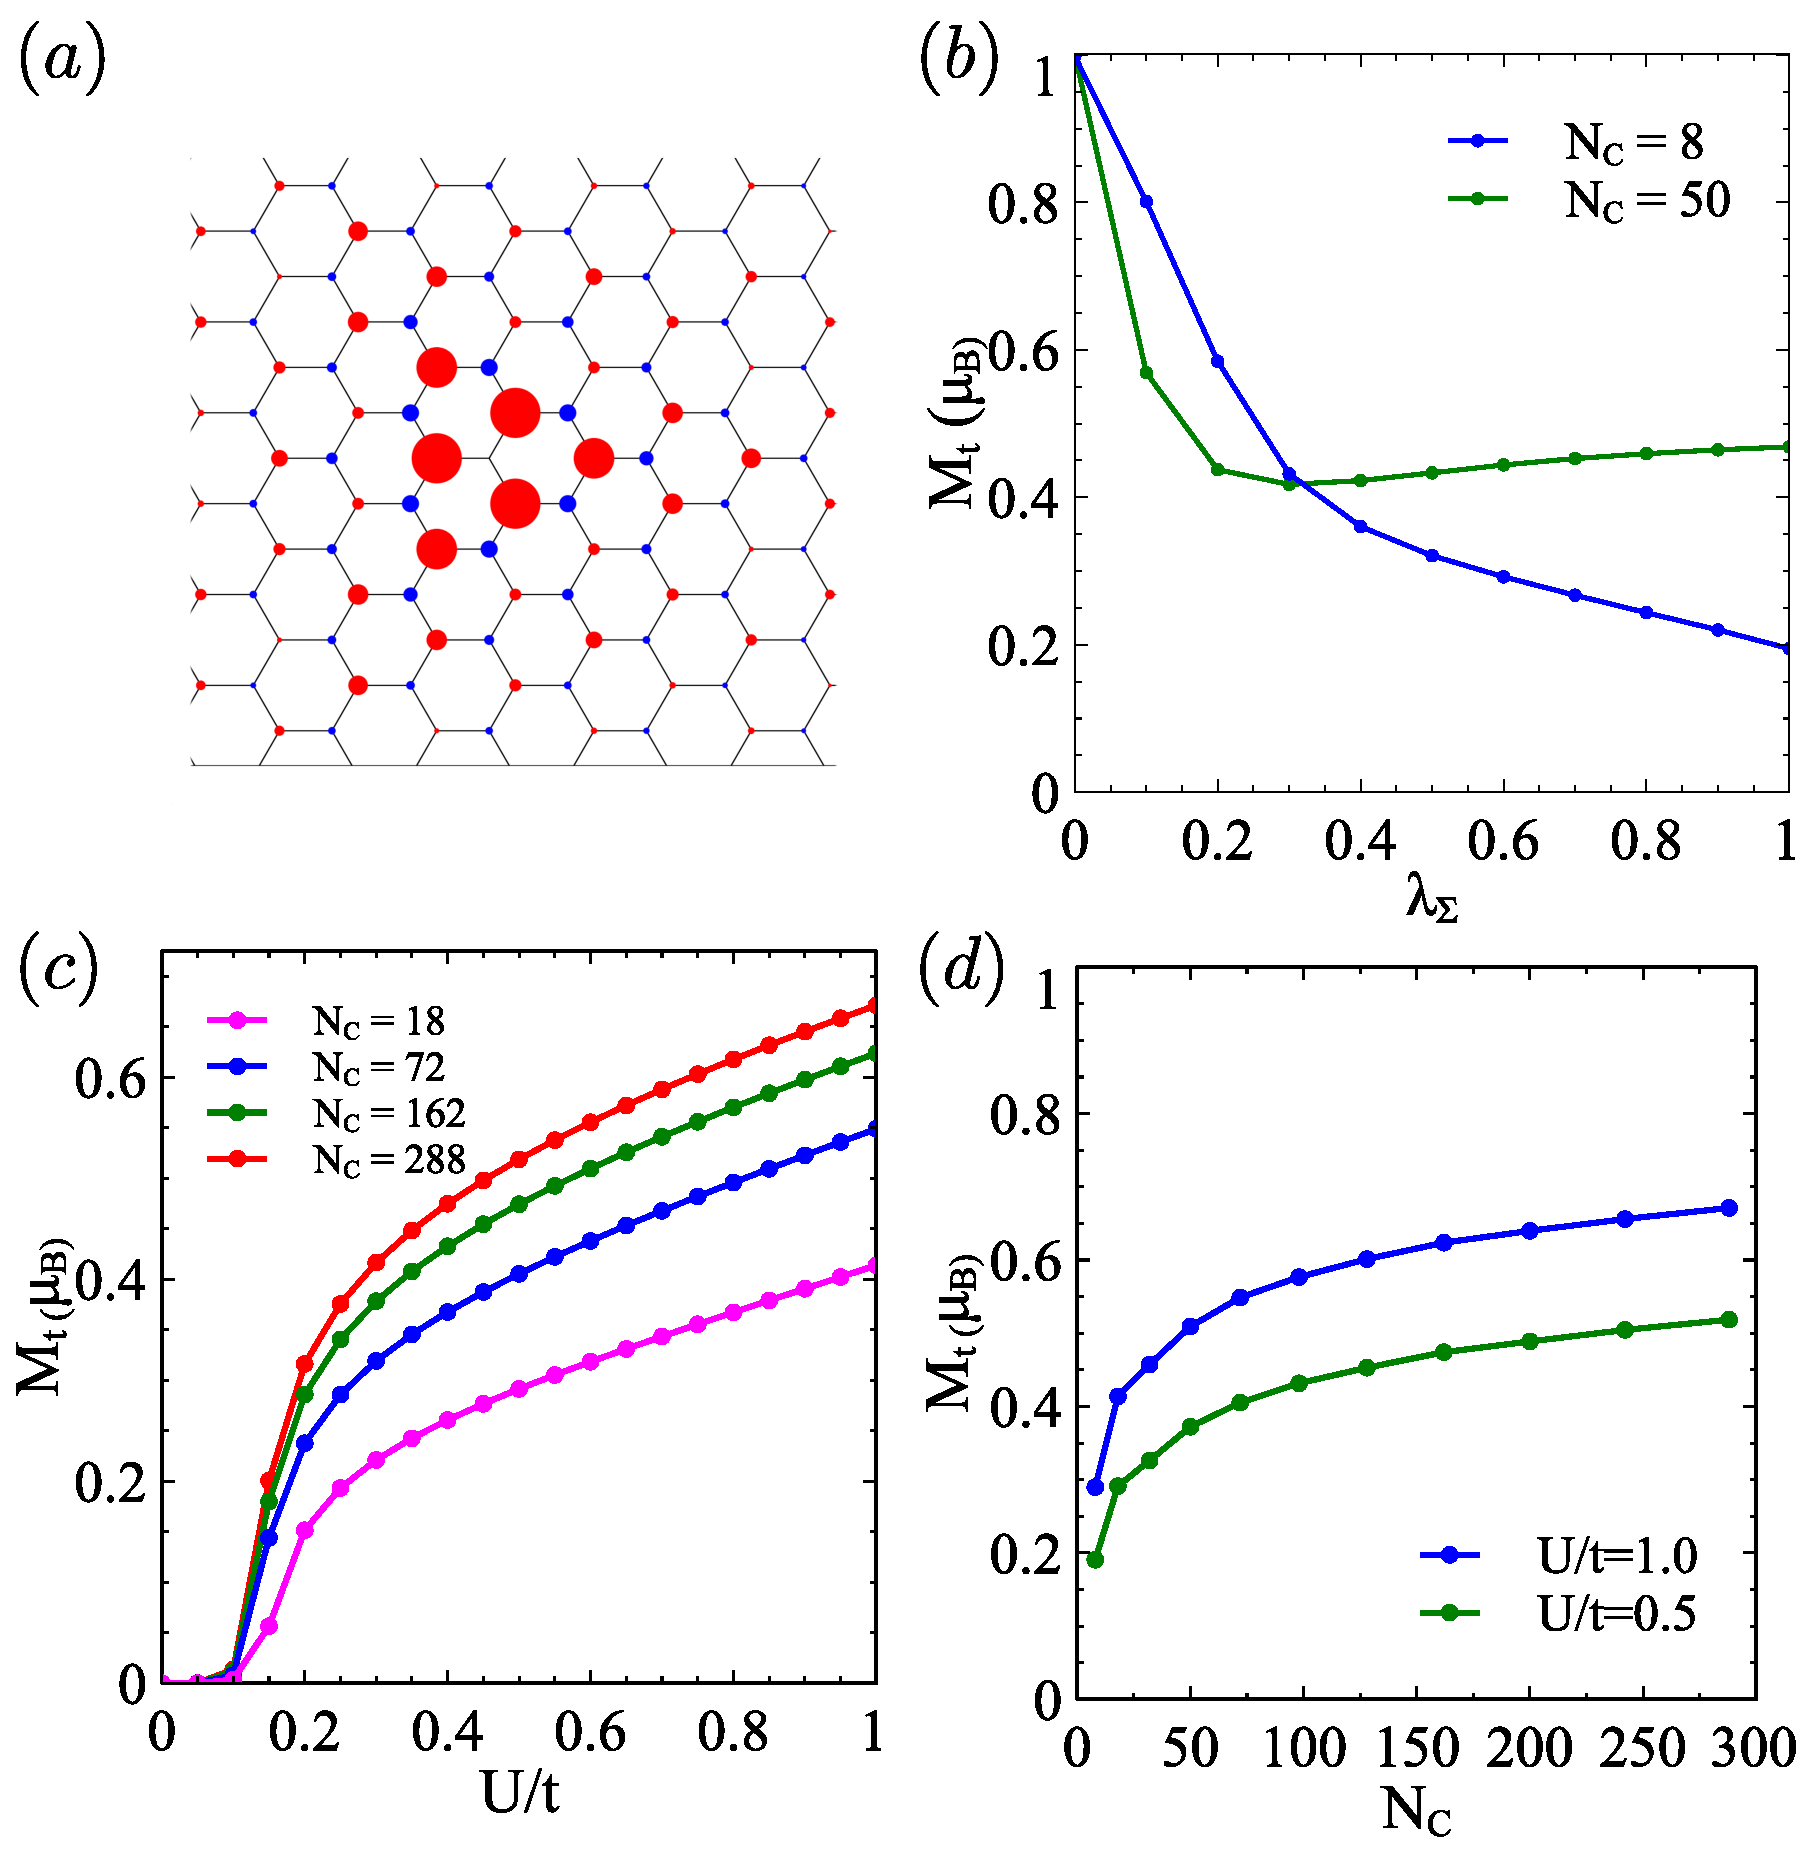
\includegraphics{chapter05/figures/figMF.pdf}
\vspace{-5pt}
\caption{$(a)$ Magnetization of an individual sp 3 functionalized system, calculated within the \ac{mf} Hubbard approximation. $(b)$ Total magnetization of the defected region as a function of its coupling to the rest of the otherwise pristine system. $(c)$ Total magnetization of the defected region as a function of the Hubbard U for different sizes of the unit cells. $(d)$ Total magnetization as a function of the size of the unit cell for two U values, notice that the magnetization is far from the expected $m = 1\mu_B$ value.}
\label{meanfield}
\end{figure}
\FloatBarrier
%~~~~~~~~~~~~~~~~~~~~~~~~~~~~~~~~~~~~~~~~~~~~~~~~~~~~~~~~~~~%
As we can see in figure \ref{meanfield}, the magnetic moment lies far from the naive 1/2 value, in fact it is not clear that in the limit of an infinitely large unit cell this value ccouldan be reached.
The study of the convergence with the size of the unit cell is the main bottleneck of this study \red{so we are not sure of its dependence}.

The embedding technique allows also the study of the soft crossover between an isolated unit cell (island) and a single defect in a pristine material. By introducing a scaling parameter we can choose the strength of the coupling between the unit cell and the surrounding environment, doing this, the equation \eqref{green} would be rewritten as
\begin{equation}
  G_A(E) = \frac{1}{E-H_{A}-\Sigma_{AB}} \quad\longrightarrow\quad
  G^{\lambda_\Sigma}_A(E) = \frac{1}{E-H_{A}-\lambda_\Sigma\Sigma_{AB}}
\end{equation}
when the parameter $\lambda_\Sigma\rightarrow0$ then the unit cell is effectively disconnected from the rest of the system, while for $\lambda_\Sigma\rightarrow1$ is normally connected. The dependence of the magnetism of the system with this parameter is shown in figure~\ref{meanfield}~(b)
%~~~~~~~~~~~~~~~~~~~~~~~~~~ FIGURE ~~~~~~~~~~~~~~~~~~~~~~~~~%
\begin{figure}[h!]
\centering
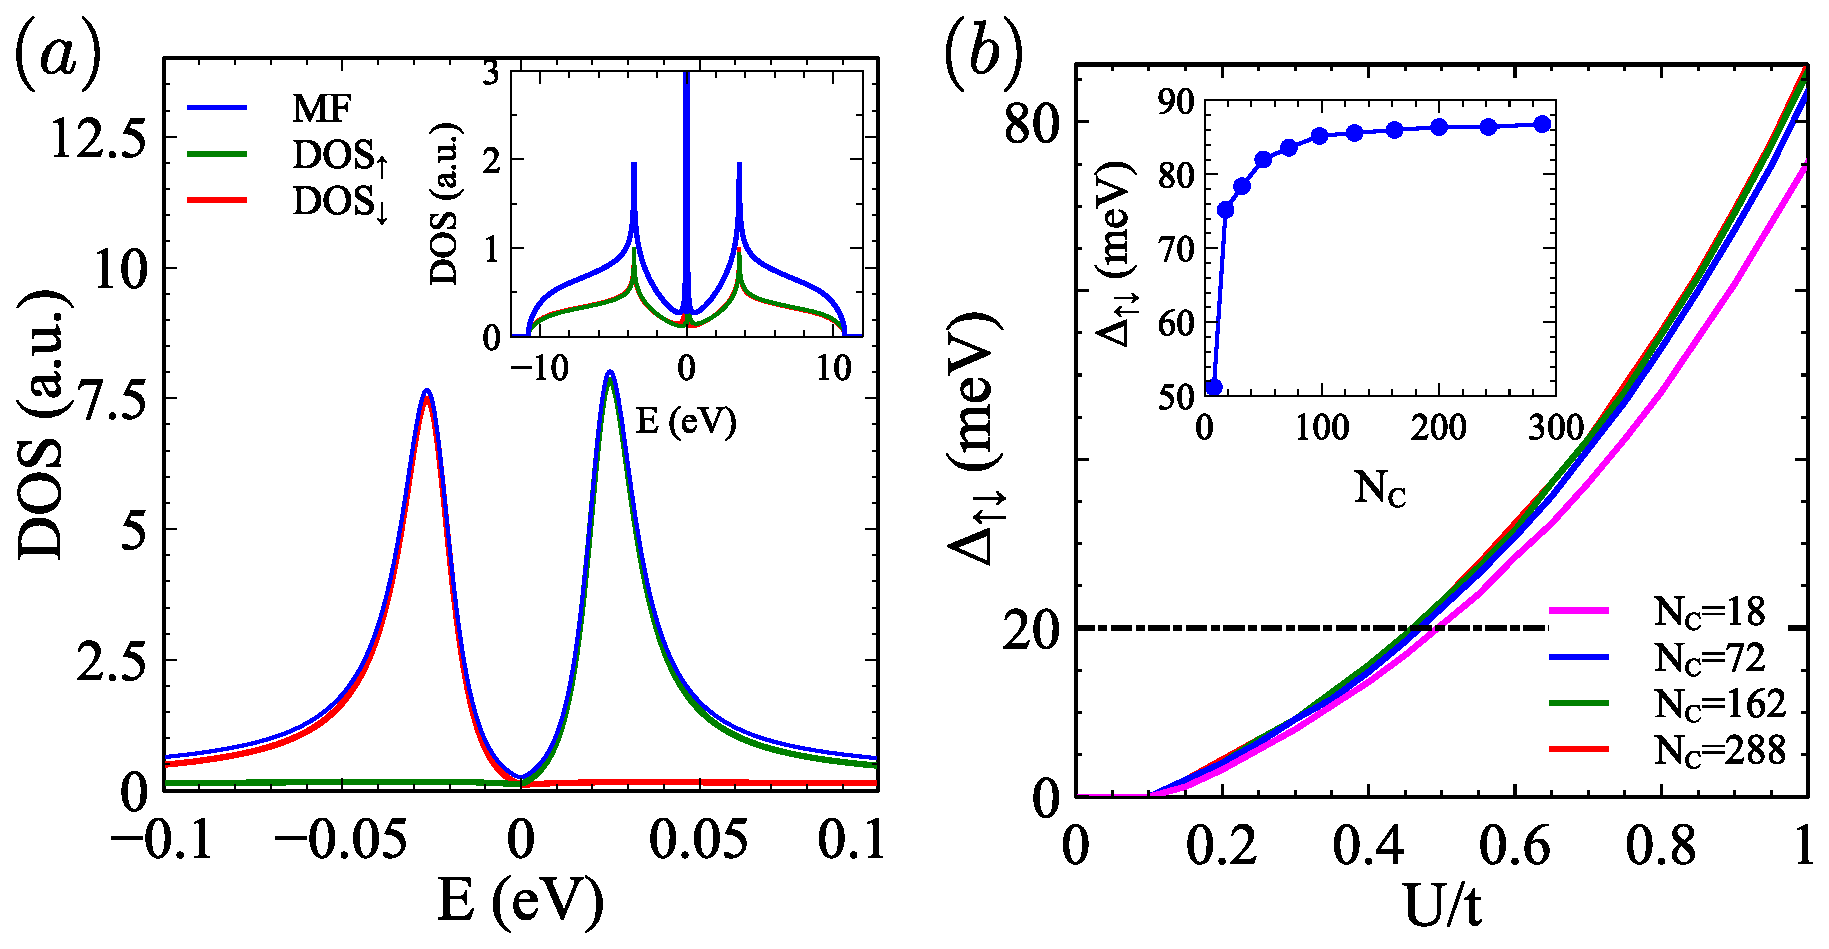
\includegraphics{chapter05/figures/MFfig2_dos.pdf}
\vspace{-5pt}
\caption{$(a)$ total and spin-resolved DOS for the Hubbard model. $(b)$ spin splitting, $\Delta$, as a function of the Hubbard interaction $U$ and, in the inset, as a function of the size of the unit cell.}
\label{coup}
\end{figure}
\FloatBarrier
%~~~~~~~~~~~~~~~~~~~~~~~~~~~~~~~~~~~~~~~~~~~~~~~~~~~~~~~~~~~%

The explanation for this behavior is that in this case we are not dealing with an isolated state in the middle of a gap ($\lambda_\Sigma=0$) which would split because of the Zeeman interaction and just by counting of the electrons would yield a magnetic moment of 1/2 at it is shown in figure \ref{coup}.
In this case we have a state that is surrounded by a continuum of states infinitesimally close even when it that happens to vanish at the exact energy of the resonance.
This is a rather pathological situation since the DOS at the energy of the ``in-gap state'' actually vanishes (like in the presence of a gap), but there are states (finite DOS) arbitrarily close to it (like in a metal). This situation is exclusive to graphene \red{(honeycomb lattice)}, and it is the main responsible for the anomalous magnetic response of the system.\\
